\documentclass[twoside]{book}

% Packages required by doxygen
\usepackage{fixltx2e}
\usepackage{calc}
\usepackage{doxygen}
\usepackage[export]{adjustbox} % also loads graphicx
\usepackage{graphicx}
\usepackage[utf8]{inputenc}
\usepackage{makeidx}
\usepackage{multicol}
\usepackage{multirow}
\PassOptionsToPackage{warn}{textcomp}
\usepackage{textcomp}
\usepackage[nointegrals]{wasysym}
\usepackage[table]{xcolor}

% Font selection
\usepackage[T1]{fontenc}
\usepackage[scaled=.90]{helvet}
\usepackage{courier}
\usepackage{amssymb}
\usepackage{sectsty}
\renewcommand{\familydefault}{\sfdefault}
\allsectionsfont{%
  \fontseries{bc}\selectfont%
  \color{darkgray}%
}
\renewcommand{\DoxyLabelFont}{%
  \fontseries{bc}\selectfont%
  \color{darkgray}%
}
\newcommand{\+}{\discretionary{\mbox{\scriptsize$\hookleftarrow$}}{}{}}

% Page & text layout
\usepackage{geometry}
\geometry{%
  a4paper,%
  top=2.5cm,%
  bottom=2.5cm,%
  left=2.5cm,%
  right=2.5cm%
}
\tolerance=750
\hfuzz=15pt
\hbadness=750
\setlength{\emergencystretch}{15pt}
\setlength{\parindent}{0cm}
\setlength{\parskip}{0.2cm}
\makeatletter
\renewcommand{\paragraph}{%
  \@startsection{paragraph}{4}{0ex}{-1.0ex}{1.0ex}{%
    \normalfont\normalsize\bfseries\SS@parafont%
  }%
}
\renewcommand{\subparagraph}{%
  \@startsection{subparagraph}{5}{0ex}{-1.0ex}{1.0ex}{%
    \normalfont\normalsize\bfseries\SS@subparafont%
  }%
}
\makeatother

% Headers & footers
\usepackage{fancyhdr}
\pagestyle{fancyplain}
\fancyhead[LE]{\fancyplain{}{\bfseries\thepage}}
\fancyhead[CE]{\fancyplain{}{}}
\fancyhead[RE]{\fancyplain{}{\bfseries\leftmark}}
\fancyhead[LO]{\fancyplain{}{\bfseries\rightmark}}
\fancyhead[CO]{\fancyplain{}{}}
\fancyhead[RO]{\fancyplain{}{\bfseries\thepage}}
\fancyfoot[LE]{\fancyplain{}{}}
\fancyfoot[CE]{\fancyplain{}{}}
\fancyfoot[RE]{\fancyplain{}{\bfseries\scriptsize Generated on Thu May 14 2015 23\+:49\+:17 for My Project by Doxygen }}
\fancyfoot[LO]{\fancyplain{}{\bfseries\scriptsize Generated on Thu May 14 2015 23\+:49\+:17 for My Project by Doxygen }}
\fancyfoot[CO]{\fancyplain{}{}}
\fancyfoot[RO]{\fancyplain{}{}}
\renewcommand{\footrulewidth}{0.4pt}
\renewcommand{\chaptermark}[1]{%
  \markboth{#1}{}%
}
\renewcommand{\sectionmark}[1]{%
  \markright{\thesection\ #1}%
}

% Indices & bibliography
\usepackage{natbib}
\usepackage[titles]{tocloft}
\setcounter{tocdepth}{3}
\setcounter{secnumdepth}{5}
\makeindex

% Hyperlinks (required, but should be loaded last)
\usepackage{ifpdf}
\ifpdf
  \usepackage[pdftex,pagebackref=true]{hyperref}
\else
  \usepackage[ps2pdf,pagebackref=true]{hyperref}
\fi
\hypersetup{%
  colorlinks=true,%
  linkcolor=blue,%
  citecolor=blue,%
  unicode%
}

% Custom commands
\newcommand{\clearemptydoublepage}{%
  \newpage{\pagestyle{empty}\cleardoublepage}%
}


%===== C O N T E N T S =====

\begin{document}

% Titlepage & ToC
\hypersetup{pageanchor=false,
             bookmarks=true,
             bookmarksnumbered=true,
             pdfencoding=unicode
            }
\pagenumbering{roman}
\begin{titlepage}
\vspace*{7cm}
\begin{center}%
{\Large My Project }\\
\vspace*{1cm}
{\large Generated by Doxygen 1.8.9.1}\\
\vspace*{0.5cm}
{\small Thu May 14 2015 23:49:17}\\
\end{center}
\end{titlepage}
\clearemptydoublepage
\tableofcontents
\clearemptydoublepage
\pagenumbering{arabic}
\hypersetup{pageanchor=true}

%--- Begin generated contents ---
\chapter{Hierarchical Index}
\section{Class Hierarchy}
This inheritance list is sorted roughly, but not completely, alphabetically\+:\begin{DoxyCompactList}
\item \contentsline{section}{Auto\+Copter}{\pageref{classAutoCopter}}{}
\item \contentsline{section}{Command}{\pageref{classCommand}}{}
\item \contentsline{section}{Command\+Input}{\pageref{classCommandInput}}{}
\begin{DoxyCompactList}
\item \contentsline{section}{Serial\+Input}{\pageref{classSerialInput}}{}
\item \contentsline{section}{S\+P\+I\+Input}{\pageref{classSPIInput}}{}
\end{DoxyCompactList}
\item \contentsline{section}{Component}{\pageref{classComponent}}{}
\begin{DoxyCompactList}
\item \contentsline{section}{E\+S\+C}{\pageref{classESC}}{}
\item \contentsline{section}{Motor}{\pageref{classMotor}}{}
\item \contentsline{section}{Sensor}{\pageref{classSensor}}{}
\begin{DoxyCompactList}
\item \contentsline{section}{Accelerometer\+Sensor}{\pageref{classAccelerometerSensor}}{}
\begin{DoxyCompactList}
\item \contentsline{section}{M\+P\+U6050}{\pageref{classMPU6050}}{}
\end{DoxyCompactList}
\item \contentsline{section}{Barometric\+Sensor}{\pageref{classBarometricSensor}}{}
\begin{DoxyCompactList}
\item \contentsline{section}{B\+M\+P180}{\pageref{classBMP180}}{}
\end{DoxyCompactList}
\item \contentsline{section}{Gyroscope\+Sensor}{\pageref{classGyroscopeSensor}}{}
\begin{DoxyCompactList}
\item \contentsline{section}{M\+P\+U6050}{\pageref{classMPU6050}}{}
\end{DoxyCompactList}
\item \contentsline{section}{Magnetometer\+Sensor}{\pageref{classMagnetometerSensor}}{}
\begin{DoxyCompactList}
\item \contentsline{section}{H\+M\+C5883\+L}{\pageref{classHMC5883L}}{}
\end{DoxyCompactList}
\end{DoxyCompactList}
\end{DoxyCompactList}
\item \contentsline{section}{E\+S\+C\+Config}{\pageref{classESCConfig}}{}
\item \contentsline{section}{Flight\+Controller}{\pageref{classFlightController}}{}
\item \contentsline{section}{G\+P\+S\+Stabilizer}{\pageref{classGPSStabilizer}}{}
\item \contentsline{section}{Parts\+List}{\pageref{classPartsList}}{}
\item \contentsline{section}{Stabilizer}{\pageref{classStabilizer}}{}
\item \contentsline{section}{Util}{\pageref{classUtil}}{}
\end{DoxyCompactList}

\chapter{Class Index}
\section{Class List}
Here are the classes, structs, unions and interfaces with brief descriptions\+:\begin{DoxyCompactList}
\item\contentsline{section}{\hyperlink{classAccelerometerSensor}{Accelerometer\+Sensor} }{\pageref{classAccelerometerSensor}}{}
\item\contentsline{section}{\hyperlink{classAutoCopter}{Auto\+Copter} }{\pageref{classAutoCopter}}{}
\item\contentsline{section}{\hyperlink{classBarometricSensor}{Barometric\+Sensor} }{\pageref{classBarometricSensor}}{}
\item\contentsline{section}{\hyperlink{classBMP180}{B\+M\+P180} }{\pageref{classBMP180}}{}
\item\contentsline{section}{\hyperlink{classCommand}{Command} }{\pageref{classCommand}}{}
\item\contentsline{section}{\hyperlink{classCommandInput}{Command\+Input} }{\pageref{classCommandInput}}{}
\item\contentsline{section}{\hyperlink{classComponent}{Component} }{\pageref{classComponent}}{}
\item\contentsline{section}{\hyperlink{classESC}{E\+S\+C} }{\pageref{classESC}}{}
\item\contentsline{section}{\hyperlink{classESCConfig}{E\+S\+C\+Config} }{\pageref{classESCConfig}}{}
\item\contentsline{section}{\hyperlink{classFlightController}{Flight\+Controller} }{\pageref{classFlightController}}{}
\item\contentsline{section}{\hyperlink{classGPSStabilizer}{G\+P\+S\+Stabilizer} }{\pageref{classGPSStabilizer}}{}
\item\contentsline{section}{\hyperlink{classGyroscopeSensor}{Gyroscope\+Sensor} }{\pageref{classGyroscopeSensor}}{}
\item\contentsline{section}{\hyperlink{classHMC5883L}{H\+M\+C5883\+L} }{\pageref{classHMC5883L}}{}
\item\contentsline{section}{\hyperlink{classMagnetometerSensor}{Magnetometer\+Sensor} }{\pageref{classMagnetometerSensor}}{}
\item\contentsline{section}{\hyperlink{classMotor}{Motor} }{\pageref{classMotor}}{}
\item\contentsline{section}{\hyperlink{classMPU6050}{M\+P\+U6050} }{\pageref{classMPU6050}}{}
\item\contentsline{section}{\hyperlink{classPartsList}{Parts\+List} }{\pageref{classPartsList}}{}
\item\contentsline{section}{\hyperlink{classSensor}{Sensor} }{\pageref{classSensor}}{}
\item\contentsline{section}{\hyperlink{classSerialInput}{Serial\+Input} }{\pageref{classSerialInput}}{}
\item\contentsline{section}{\hyperlink{classSPIInput}{S\+P\+I\+Input} }{\pageref{classSPIInput}}{}
\item\contentsline{section}{\hyperlink{classStabilizer}{Stabilizer} }{\pageref{classStabilizer}}{}
\item\contentsline{section}{\hyperlink{classUtil}{Util} }{\pageref{classUtil}}{}
\end{DoxyCompactList}

\chapter{File Index}
\section{File List}
Here is a list of all documented files with brief descriptions\+:\begin{DoxyCompactList}
\item\contentsline{section}{src/\+Commands/{\bfseries Command.\+h} }{\pageref{Command_8h}}{}
\item\contentsline{section}{src/\+Commands/\hyperlink{Protocol_8h}{Protocol.\+h} }{\pageref{Protocol_8h}}{}
\item\contentsline{section}{src/\+Commands/\+Command\+Input/\hyperlink{CommandInput_8cpp}{Command\+Input.\+cpp} }{\pageref{CommandInput_8cpp}}{}
\item\contentsline{section}{src/\+Commands/\+Command\+Input/\hyperlink{CommandInput_8h}{Command\+Input.\+h} }{\pageref{CommandInput_8h}}{}
\item\contentsline{section}{src/\+Commands/\+Command\+Input/\+Inputs/\hyperlink{SerialInput_8cpp}{Serial\+Input.\+cpp} }{\pageref{SerialInput_8cpp}}{}
\item\contentsline{section}{src/\+Commands/\+Command\+Input/\+Inputs/\hyperlink{SerialInput_8h}{Serial\+Input.\+h} }{\pageref{SerialInput_8h}}{}
\item\contentsline{section}{src/\+Commands/\+Command\+Input/\+Inputs/\hyperlink{SPIInput_8cpp}{S\+P\+I\+Input.\+cpp} }{\pageref{SPIInput_8cpp}}{}
\item\contentsline{section}{src/\+Commands/\+Command\+Input/\+Inputs/\hyperlink{SPIInput_8h}{S\+P\+I\+Input.\+h} }{\pageref{SPIInput_8h}}{}
\item\contentsline{section}{src/\+Components/\hyperlink{Component_8cpp}{Component.\+cpp} }{\pageref{Component_8cpp}}{}
\item\contentsline{section}{src/\+Components/\hyperlink{Component_8h}{Component.\+h} }{\pageref{Component_8h}}{}
\item\contentsline{section}{src/\+Components/\+E\+S\+C/\hyperlink{ESC_8cpp}{E\+S\+C.\+cpp} }{\pageref{ESC_8cpp}}{}
\item\contentsline{section}{src/\+Components/\+E\+S\+C/\hyperlink{ESC_8h}{E\+S\+C.\+h} }{\pageref{ESC_8h}}{}
\item\contentsline{section}{src/\+Components/\+E\+S\+C/\hyperlink{ESCConfig_8cpp}{E\+S\+C\+Config.\+cpp} }{\pageref{ESCConfig_8cpp}}{}
\item\contentsline{section}{src/\+Components/\+E\+S\+C/\hyperlink{ESCConfig_8h}{E\+S\+C\+Config.\+h} }{\pageref{ESCConfig_8h}}{}
\item\contentsline{section}{src/\+Components/\+Motor/\hyperlink{Motor_8cpp}{Motor.\+cpp} }{\pageref{Motor_8cpp}}{}
\item\contentsline{section}{src/\+Components/\+Motor/\hyperlink{Motor_8h}{Motor.\+h} }{\pageref{Motor_8h}}{}
\item\contentsline{section}{src/\+Components/\+Parts/\hyperlink{PartsList_8cpp}{Parts\+List.\+cpp} }{\pageref{PartsList_8cpp}}{}
\item\contentsline{section}{src/\+Components/\+Parts/\hyperlink{PartsList_8h}{Parts\+List.\+h} }{\pageref{PartsList_8h}}{}
\item\contentsline{section}{src/\+Components/\+Parts/\+B\+M\+P180/\hyperlink{BMP180_8cpp}{B\+M\+P180.\+cpp} }{\pageref{BMP180_8cpp}}{}
\item\contentsline{section}{src/\+Components/\+Parts/\+B\+M\+P180/\hyperlink{BMP180_8h}{B\+M\+P180.\+h} }{\pageref{BMP180_8h}}{}
\item\contentsline{section}{src/\+Components/\+Parts/\+H\+M\+C5883\+L/\hyperlink{HMC5883L_8cpp}{H\+M\+C5883\+L.\+cpp} }{\pageref{HMC5883L_8cpp}}{}
\item\contentsline{section}{src/\+Components/\+Parts/\+H\+M\+C5883\+L/\hyperlink{HMC5883L_8h}{H\+M\+C5883\+L.\+h} }{\pageref{HMC5883L_8h}}{}
\item\contentsline{section}{src/\+Components/\+Parts/\+M\+P\+U6050/\hyperlink{MPU6050_8cpp}{M\+P\+U6050.\+cpp} }{\pageref{MPU6050_8cpp}}{}
\item\contentsline{section}{src/\+Components/\+Parts/\+M\+P\+U6050/\hyperlink{MPU6050_8h}{M\+P\+U6050.\+h} }{\pageref{MPU6050_8h}}{}
\item\contentsline{section}{src/\+Components/\+Sensor/\hyperlink{Sensor_8cpp}{Sensor.\+cpp} }{\pageref{Sensor_8cpp}}{}
\item\contentsline{section}{src/\+Components/\+Sensor/\hyperlink{Sensor_8h}{Sensor.\+h} }{\pageref{Sensor_8h}}{}
\item\contentsline{section}{src/\+Components/\+Sensor/\+Accelerometer\+Sensor/\hyperlink{AccelerometerSensor_8cpp}{Accelerometer\+Sensor.\+cpp} }{\pageref{AccelerometerSensor_8cpp}}{}
\item\contentsline{section}{src/\+Components/\+Sensor/\+Accelerometer\+Sensor/\hyperlink{AccelerometerSensor_8h}{Accelerometer\+Sensor.\+h} }{\pageref{AccelerometerSensor_8h}}{}
\item\contentsline{section}{src/\+Components/\+Sensor/\+Barometer\+Sensor/\hyperlink{BarometricSensor_8cpp}{Barometric\+Sensor.\+cpp} }{\pageref{BarometricSensor_8cpp}}{}
\item\contentsline{section}{src/\+Components/\+Sensor/\+Barometer\+Sensor/\hyperlink{BarometricSensor_8h}{Barometric\+Sensor.\+h} }{\pageref{BarometricSensor_8h}}{}
\item\contentsline{section}{src/\+Components/\+Sensor/\+Gyroscope\+Sensor/\hyperlink{GyroscopeSensor_8cpp}{Gyroscope\+Sensor.\+cpp} }{\pageref{GyroscopeSensor_8cpp}}{}
\item\contentsline{section}{src/\+Components/\+Sensor/\+Gyroscope\+Sensor/\hyperlink{GyroscopeSensor_8h}{Gyroscope\+Sensor.\+h} }{\pageref{GyroscopeSensor_8h}}{}
\item\contentsline{section}{src/\+Components/\+Sensor/\+Magnetometer\+Sensor/\hyperlink{MagnetometerSensor_8cpp}{Magnetometer\+Sensor.\+cpp} }{\pageref{MagnetometerSensor_8cpp}}{}
\item\contentsline{section}{src/\+Components/\+Sensor/\+Magnetometer\+Sensor/\hyperlink{MagnetometerSensor_8h}{Magnetometer\+Sensor.\+h} }{\pageref{MagnetometerSensor_8h}}{}
\item\contentsline{section}{src/\+Flight\+Controller/\hyperlink{FlightController_8cpp}{Flight\+Controller.\+cpp} }{\pageref{FlightController_8cpp}}{}
\item\contentsline{section}{src/\+Flight\+Controller/\hyperlink{FlightController_8h}{Flight\+Controller.\+h} }{\pageref{FlightController_8h}}{}
\item\contentsline{section}{src/\+Flight\+Controller/\+Stabilizer/{\bfseries Stabilizer.\+h} }{\pageref{Stabilizer_8h}}{}
\item\contentsline{section}{src/\+Flight\+Controller/\+Stabilizer/\+Stabilizers/{\bfseries G\+P\+S\+Stabilizer.\+h} }{\pageref{GPSStabilizer_8h}}{}
\item\contentsline{section}{src/\+Main/\hyperlink{AutoCopter_8cpp}{Auto\+Copter.\+cpp} }{\pageref{AutoCopter_8cpp}}{}
\item\contentsline{section}{src/\+Main/\hyperlink{AutoCopter_8h}{Auto\+Copter.\+h} }{\pageref{AutoCopter_8h}}{}
\item\contentsline{section}{src/\+Util/\hyperlink{Util_8cpp}{Util.\+cpp} }{\pageref{Util_8cpp}}{}
\item\contentsline{section}{src/\+Util/\hyperlink{Util_8h}{Util.\+h} }{\pageref{Util_8h}}{}
\end{DoxyCompactList}

\chapter{Class Documentation}
\hypertarget{classAccelerometerSensor}{}\section{Accelerometer\+Sensor Class Reference}
\label{classAccelerometerSensor}\index{Accelerometer\+Sensor@{Accelerometer\+Sensor}}
Inheritance diagram for Accelerometer\+Sensor\+:\begin{figure}[H]
\begin{center}
\leavevmode
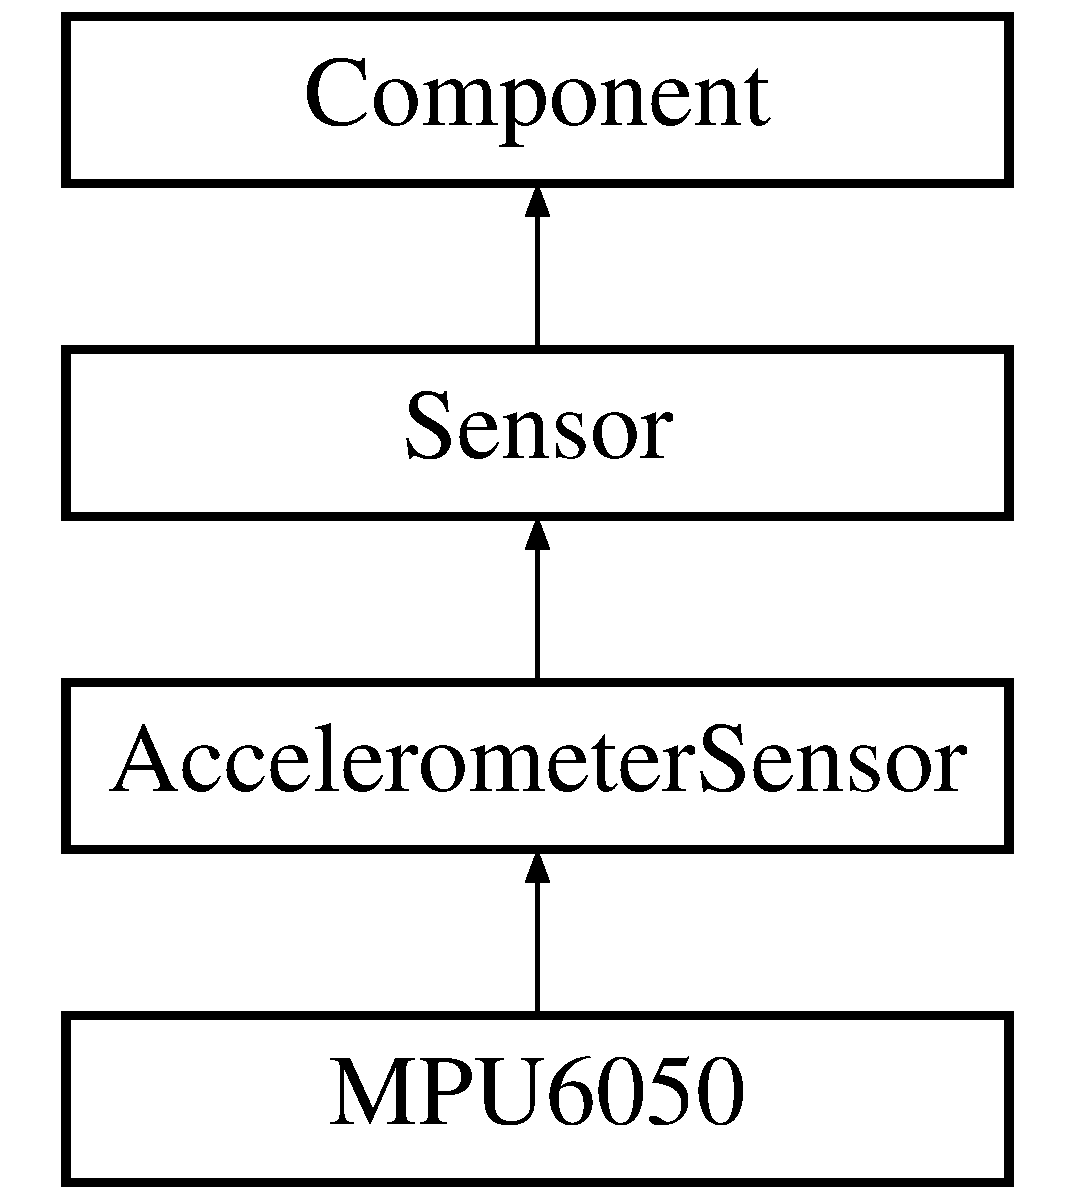
\includegraphics[height=4.000000cm]{classAccelerometerSensor}
\end{center}
\end{figure}
\subsection*{Additional Inherited Members}


The documentation for this class was generated from the following files\+:\begin{DoxyCompactItemize}
\item 
src/\+Components/\+Sensor/\+Accelerometer\+Sensor/\hyperlink{AccelerometerSensor_8h}{Accelerometer\+Sensor.\+h}\item 
src/\+Components/\+Sensor/\+Accelerometer\+Sensor/\hyperlink{AccelerometerSensor_8cpp}{Accelerometer\+Sensor.\+cpp}\end{DoxyCompactItemize}

\hypertarget{classAutoCopter}{}\section{Auto\+Copter Class Reference}
\label{classAutoCopter}\index{Auto\+Copter@{Auto\+Copter}}


{\ttfamily \#include $<$Auto\+Copter.\+h$>$}

\subsection*{Public Member Functions}
\begin{DoxyCompactItemize}
\item 
\hyperlink{classAutoCopter_a527ad0ed7b5e4c3b9bb0d748638064ef}{Auto\+Copter} (const \hyperlink{classPartsList}{Parts\+List} \&parts\+List, const \hyperlink{classFlightController}{Flight\+Controller} \&flight\+Controller)
\item 
void \hyperlink{classAutoCopter_aac4b3c3e43e2bb72136ccc8491b9b545}{setup} ()
\item 
void \hyperlink{classAutoCopter_a54f2d2f24ca0323fdb12ba6e3dc7f600}{loop} ()
\end{DoxyCompactItemize}


\subsection{Detailed Description}
Thin class over Autocopter.\+ino. Created solely for Doxygen ease of use. 

\subsection{Constructor \& Destructor Documentation}
\hypertarget{classAutoCopter_a527ad0ed7b5e4c3b9bb0d748638064ef}{}\index{Auto\+Copter@{Auto\+Copter}!Auto\+Copter@{Auto\+Copter}}
\index{Auto\+Copter@{Auto\+Copter}!Auto\+Copter@{Auto\+Copter}}
\subsubsection[{Auto\+Copter(const Parts\+List \&parts\+List, const Flight\+Controller \&flight\+Controller)}]{\setlength{\rightskip}{0pt plus 5cm}Auto\+Copter\+::\+Auto\+Copter (
\begin{DoxyParamCaption}
\item[{const {\bf Parts\+List} \&}]{parts\+List, }
\item[{const {\bf Flight\+Controller} \&}]{flight\+Controller}
\end{DoxyParamCaption}
)}\label{classAutoCopter_a527ad0ed7b5e4c3b9bb0d748638064ef}
Construct our Copter with a list of Parts and \hyperlink{classFlightController}{Flight\+Controller} 

\subsection{Member Function Documentation}
\hypertarget{classAutoCopter_a54f2d2f24ca0323fdb12ba6e3dc7f600}{}\index{Auto\+Copter@{Auto\+Copter}!loop@{loop}}
\index{loop@{loop}!Auto\+Copter@{Auto\+Copter}}
\subsubsection[{loop()}]{\setlength{\rightskip}{0pt plus 5cm}void Auto\+Copter\+::loop (
\begin{DoxyParamCaption}
{}
\end{DoxyParamCaption}
)}\label{classAutoCopter_a54f2d2f24ca0323fdb12ba6e3dc7f600}
Basic flight loop.
\begin{DoxyEnumerate}
\item Get a command
\item If command -\/$>$ do it
\end{DoxyEnumerate}
\begin{DoxyEnumerate}
\item Else -\/$>$ Stabilize using a \hyperlink{classStabilizer}{Stabilizer} if available 
\end{DoxyEnumerate}\hypertarget{classAutoCopter_aac4b3c3e43e2bb72136ccc8491b9b545}{}\index{Auto\+Copter@{Auto\+Copter}!setup@{setup}}
\index{setup@{setup}!Auto\+Copter@{Auto\+Copter}}
\subsubsection[{setup()}]{\setlength{\rightskip}{0pt plus 5cm}void Auto\+Copter\+::setup (
\begin{DoxyParamCaption}
{}
\end{DoxyParamCaption}
)}\label{classAutoCopter_aac4b3c3e43e2bb72136ccc8491b9b545}
Setup various parts in our Parts List. Then run some basic tests, if specified. 

The documentation for this class was generated from the following files\+:\begin{DoxyCompactItemize}
\item 
src/\+Main/\hyperlink{AutoCopter_8h}{Auto\+Copter.\+h}\item 
src/\+Main/\hyperlink{AutoCopter_8cpp}{Auto\+Copter.\+cpp}\end{DoxyCompactItemize}

\hypertarget{classBarometricSensor}{}\section{Barometric\+Sensor Class Reference}
\label{classBarometricSensor}\index{Barometric\+Sensor@{Barometric\+Sensor}}


{\ttfamily \#include $<$Barometric\+Sensor.\+h$>$}

Inheritance diagram for Barometric\+Sensor\+:\begin{figure}[H]
\begin{center}
\leavevmode
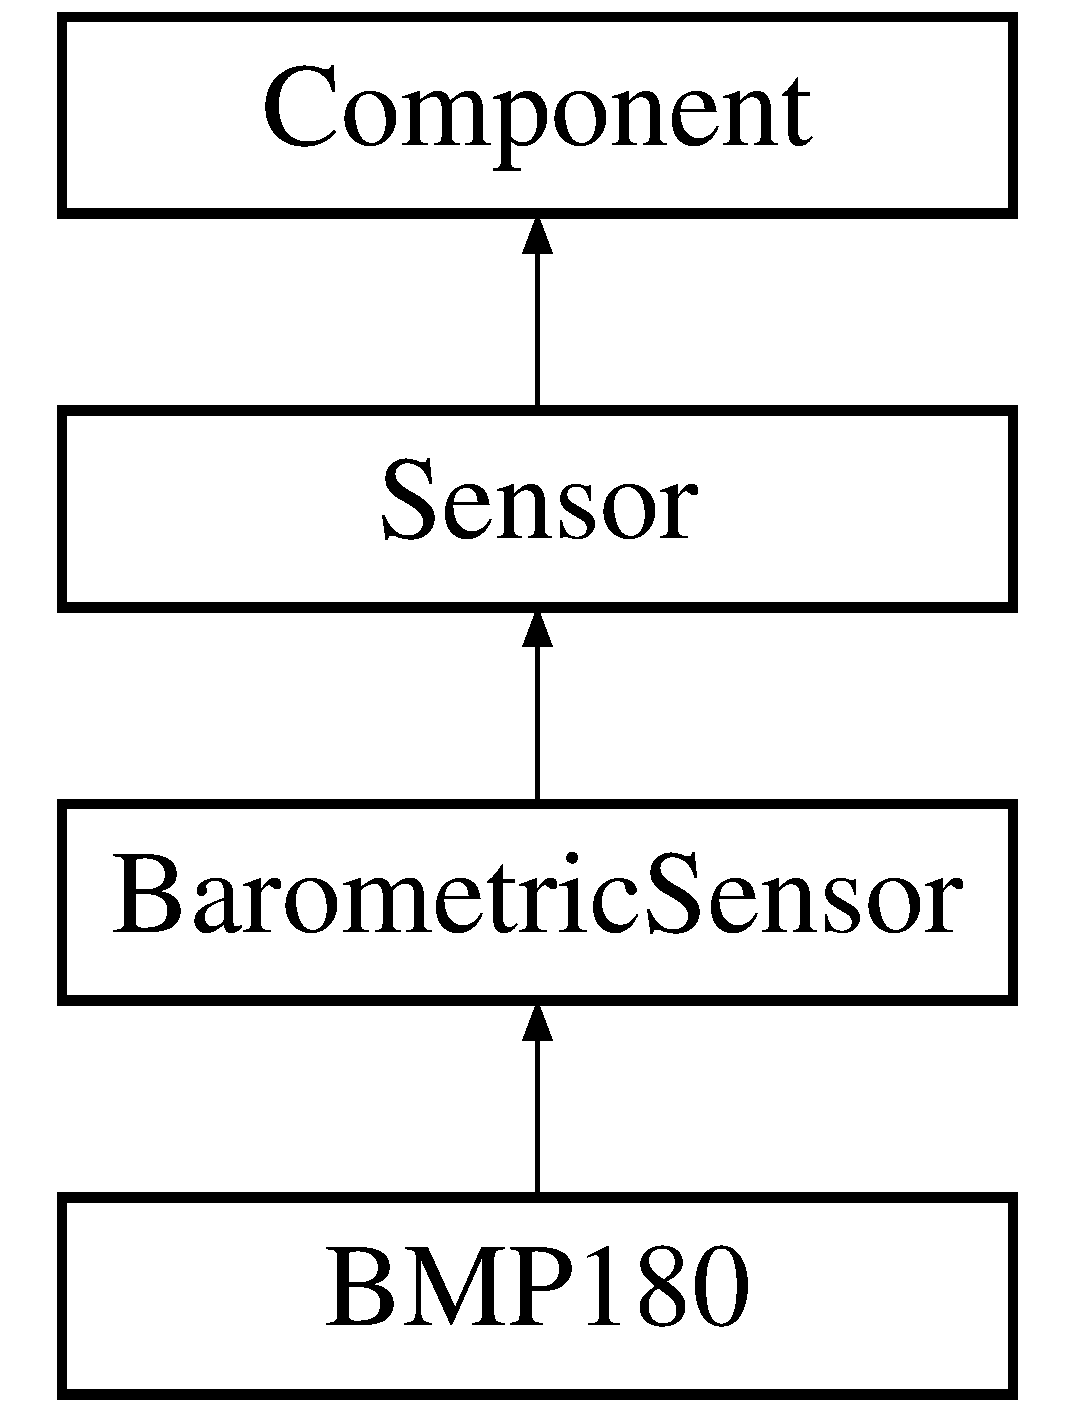
\includegraphics[height=4.000000cm]{classBarometricSensor}
\end{center}
\end{figure}
\subsection*{Public Member Functions}
\begin{DoxyCompactItemize}
\item 
\hyperlink{classBarometricSensor_ab61cf4c4713a6f7fa2a29e95096b21f5}{Barometric\+Sensor} ()
\item 
virtual \hyperlink{classBarometricSensor_a17f40d7055700aa4feedc0755485d5d4}{$\sim$\+Barometric\+Sensor} ()
\item 
\hypertarget{classBarometricSensor_a9f7875e4509fb9c57df9eddc76de993e}{}void {\bfseries update\+Readings} ()\label{classBarometricSensor_a9f7875e4509fb9c57df9eddc76de993e}

\item 
float \hyperlink{classBarometricSensor_a7a4c8a68ebf409ea53baf36c9344307f}{get\+Pressure} ()
\end{DoxyCompactItemize}


\subsection{Detailed Description}
This virtual class represents the concept of a \hyperlink{classBarometricSensor}{Barometric\+Sensor} because this piece could be combined with other hardware. 

\subsection{Constructor \& Destructor Documentation}
\hypertarget{classBarometricSensor_ab61cf4c4713a6f7fa2a29e95096b21f5}{}\index{Barometric\+Sensor@{Barometric\+Sensor}!Barometric\+Sensor@{Barometric\+Sensor}}
\index{Barometric\+Sensor@{Barometric\+Sensor}!Barometric\+Sensor@{Barometric\+Sensor}}
\subsubsection[{Barometric\+Sensor()}]{\setlength{\rightskip}{0pt plus 5cm}Barometric\+Sensor\+::\+Barometric\+Sensor (
\begin{DoxyParamCaption}
{}
\end{DoxyParamCaption}
)}\label{classBarometricSensor_ab61cf4c4713a6f7fa2a29e95096b21f5}
Construct a new \hyperlink{classBarometricSensor}{Barometric\+Sensor} with the given name. \hypertarget{classBarometricSensor_a17f40d7055700aa4feedc0755485d5d4}{}\index{Barometric\+Sensor@{Barometric\+Sensor}!````~Barometric\+Sensor@{$\sim$\+Barometric\+Sensor}}
\index{````~Barometric\+Sensor@{$\sim$\+Barometric\+Sensor}!Barometric\+Sensor@{Barometric\+Sensor}}
\subsubsection[{$\sim$\+Barometric\+Sensor()}]{\setlength{\rightskip}{0pt plus 5cm}Barometric\+Sensor\+::$\sim$\+Barometric\+Sensor (
\begin{DoxyParamCaption}
{}
\end{DoxyParamCaption}
)\hspace{0.3cm}{\ttfamily [virtual]}}\label{classBarometricSensor_a17f40d7055700aa4feedc0755485d5d4}
Unused 

\subsection{Member Function Documentation}
\hypertarget{classBarometricSensor_a7a4c8a68ebf409ea53baf36c9344307f}{}\index{Barometric\+Sensor@{Barometric\+Sensor}!get\+Pressure@{get\+Pressure}}
\index{get\+Pressure@{get\+Pressure}!Barometric\+Sensor@{Barometric\+Sensor}}
\subsubsection[{get\+Pressure()}]{\setlength{\rightskip}{0pt plus 5cm}float Barometric\+Sensor\+::get\+Pressure (
\begin{DoxyParamCaption}
{}
\end{DoxyParamCaption}
)}\label{classBarometricSensor_a7a4c8a68ebf409ea53baf36c9344307f}
Read the last updated pressure value 

The documentation for this class was generated from the following files\+:\begin{DoxyCompactItemize}
\item 
src/\+Components/\+Sensor/\+Barometer\+Sensor/\hyperlink{BarometricSensor_8h}{Barometric\+Sensor.\+h}\item 
src/\+Components/\+Sensor/\+Barometer\+Sensor/\hyperlink{BarometricSensor_8cpp}{Barometric\+Sensor.\+cpp}\end{DoxyCompactItemize}

\hypertarget{classBMP180}{}\section{B\+M\+P180 Class Reference}
\label{classBMP180}\index{B\+M\+P180@{B\+M\+P180}}


{\ttfamily \#include $<$B\+M\+P180.\+h$>$}

Inheritance diagram for B\+M\+P180\+:\begin{figure}[H]
\begin{center}
\leavevmode
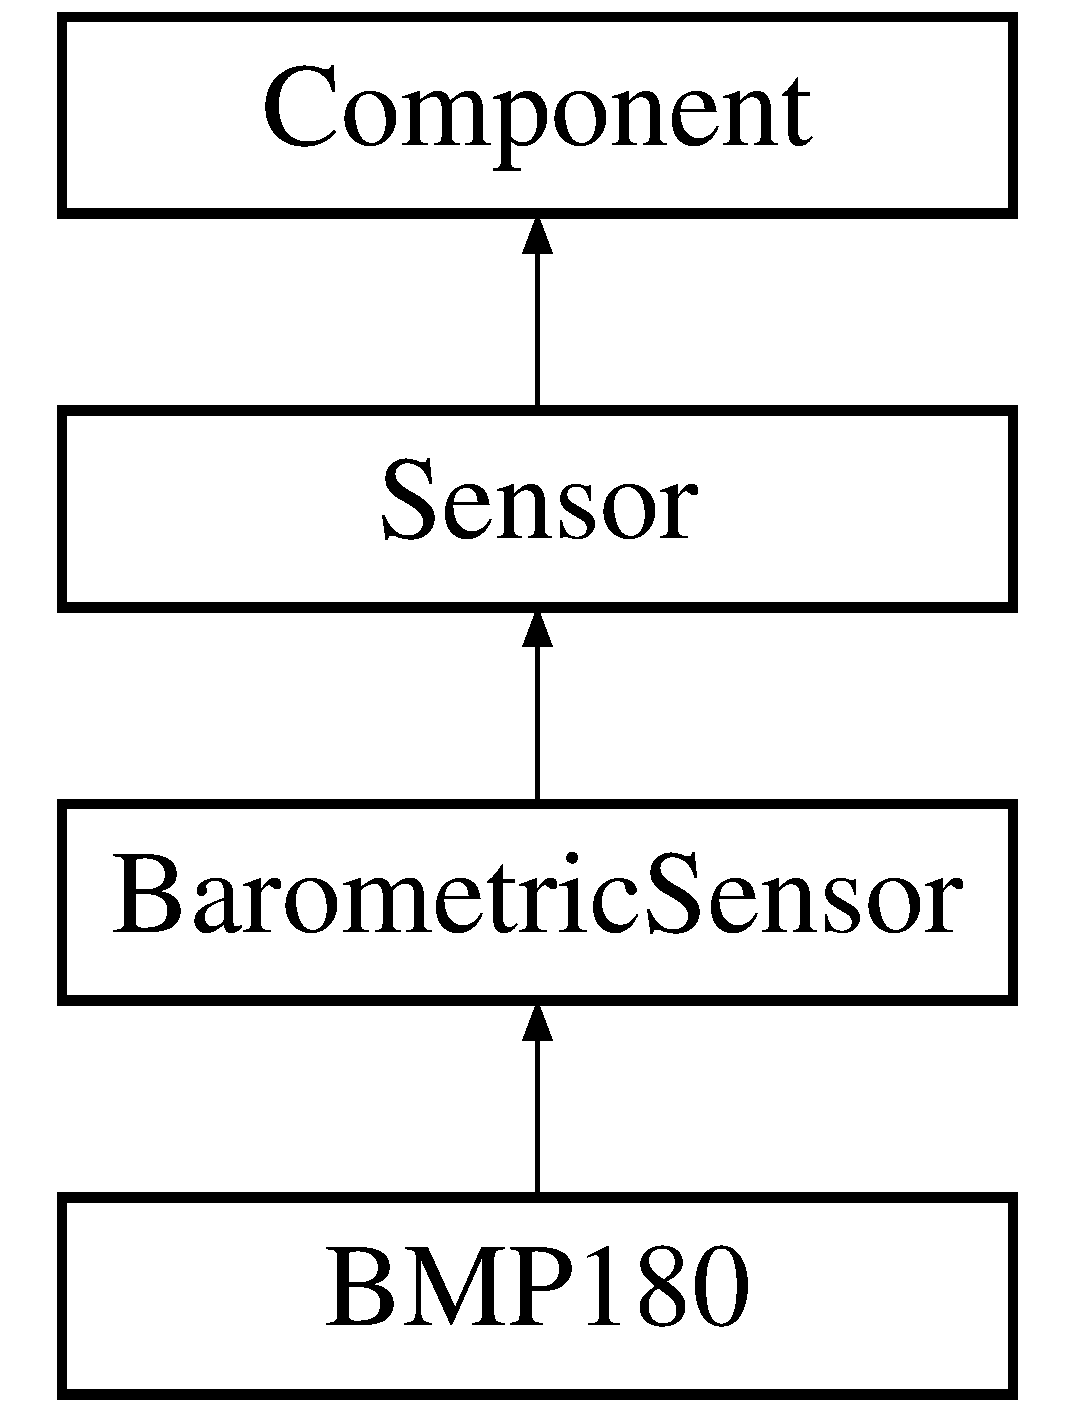
\includegraphics[height=4.000000cm]{classBMP180}
\end{center}
\end{figure}
\subsection*{Public Member Functions}
\begin{DoxyCompactItemize}
\item 
\hyperlink{classBMP180_a8c3e89c7ea65e49c0001a43af07b7c35}{B\+M\+P180} ()
\item 
virtual \hyperlink{classBMP180_a8d434a3074ba607d2dbc14657ae224dd}{$\sim$\+B\+M\+P180} ()
\item 
String \hyperlink{classBMP180_a5d119ee8ca9d113dba19199e7614161a}{get\+Logging\+Info} ()
\item 
void \hyperlink{classBMP180_a901de95ff24e96876ba0016a848cb955}{update\+Readings} ()
\end{DoxyCompactItemize}


\subsection{Detailed Description}
This class represents the specific piece of hardware\+: \hyperlink{classBMP180}{B\+M\+P180} 

\subsection{Constructor \& Destructor Documentation}
\hypertarget{classBMP180_a8c3e89c7ea65e49c0001a43af07b7c35}{}\index{B\+M\+P180@{B\+M\+P180}!B\+M\+P180@{B\+M\+P180}}
\index{B\+M\+P180@{B\+M\+P180}!B\+M\+P180@{B\+M\+P180}}
\subsubsection[{B\+M\+P180()}]{\setlength{\rightskip}{0pt plus 5cm}B\+M\+P180\+::\+B\+M\+P180 (
\begin{DoxyParamCaption}
{}
\end{DoxyParamCaption}
)}\label{classBMP180_a8c3e89c7ea65e49c0001a43af07b7c35}
Construct a new \hyperlink{classBMP180}{B\+M\+P180} \hypertarget{classBMP180_a8d434a3074ba607d2dbc14657ae224dd}{}\index{B\+M\+P180@{B\+M\+P180}!````~B\+M\+P180@{$\sim$\+B\+M\+P180}}
\index{````~B\+M\+P180@{$\sim$\+B\+M\+P180}!B\+M\+P180@{B\+M\+P180}}
\subsubsection[{$\sim$\+B\+M\+P180()}]{\setlength{\rightskip}{0pt plus 5cm}B\+M\+P180\+::$\sim$\+B\+M\+P180 (
\begin{DoxyParamCaption}
{}
\end{DoxyParamCaption}
)\hspace{0.3cm}{\ttfamily [virtual]}}\label{classBMP180_a8d434a3074ba607d2dbc14657ae224dd}
Unused 

\subsection{Member Function Documentation}
\hypertarget{classBMP180_a5d119ee8ca9d113dba19199e7614161a}{}\index{B\+M\+P180@{B\+M\+P180}!get\+Logging\+Info@{get\+Logging\+Info}}
\index{get\+Logging\+Info@{get\+Logging\+Info}!B\+M\+P180@{B\+M\+P180}}
\subsubsection[{get\+Logging\+Info()}]{\setlength{\rightskip}{0pt plus 5cm}String B\+M\+P180\+::get\+Logging\+Info (
\begin{DoxyParamCaption}
{}
\end{DoxyParamCaption}
)}\label{classBMP180_a5d119ee8ca9d113dba19199e7614161a}
Return a non-\/newline ended string containing information about the \hyperlink{classComponent}{Component} \hypertarget{classBMP180_a901de95ff24e96876ba0016a848cb955}{}\index{B\+M\+P180@{B\+M\+P180}!update\+Readings@{update\+Readings}}
\index{update\+Readings@{update\+Readings}!B\+M\+P180@{B\+M\+P180}}
\subsubsection[{update\+Readings()}]{\setlength{\rightskip}{0pt plus 5cm}void B\+M\+P180\+::update\+Readings (
\begin{DoxyParamCaption}
{}
\end{DoxyParamCaption}
)\hspace{0.3cm}{\ttfamily [virtual]}}\label{classBMP180_a901de95ff24e96876ba0016a848cb955}
Updates the current pressure reading 

Reimplemented from \hyperlink{classBarometricSensor}{Barometric\+Sensor}.



The documentation for this class was generated from the following files\+:\begin{DoxyCompactItemize}
\item 
src/\+Components/\+Parts/\+B\+M\+P180/\hyperlink{BMP180_8h}{B\+M\+P180.\+h}\item 
src/\+Components/\+Parts/\+B\+M\+P180/\hyperlink{BMP180_8cpp}{B\+M\+P180.\+cpp}\end{DoxyCompactItemize}

\hypertarget{classCommand}{}\section{Command Class Reference}
\label{classCommand}\index{Command@{Command}}
\subsection*{Public Member Functions}
\begin{DoxyCompactItemize}
\item 
\hypertarget{classCommand_aa8f47dd5fd5fad41ac703e25ae0a120c}{}{\bfseries Command} (\hyperlink{Protocol_8h_a0fbada5bff0eeb4dc6be4b6e6f1c4eaf}{C\+O\+M\+M\+A\+N\+D} command, int scalar)\label{classCommand_aa8f47dd5fd5fad41ac703e25ae0a120c}

\end{DoxyCompactItemize}


The documentation for this class was generated from the following files\+:\begin{DoxyCompactItemize}
\item 
src/\+Commands/Command.\+h\item 
src/\+Commands/Command.\+cpp\end{DoxyCompactItemize}

\hypertarget{classCommandInput}{}\section{Command\+Input Class Reference}
\label{classCommandInput}\index{Command\+Input@{Command\+Input}}


{\ttfamily \#include $<$Command\+Input.\+h$>$}

Inheritance diagram for Command\+Input\+:\begin{figure}[H]
\begin{center}
\leavevmode
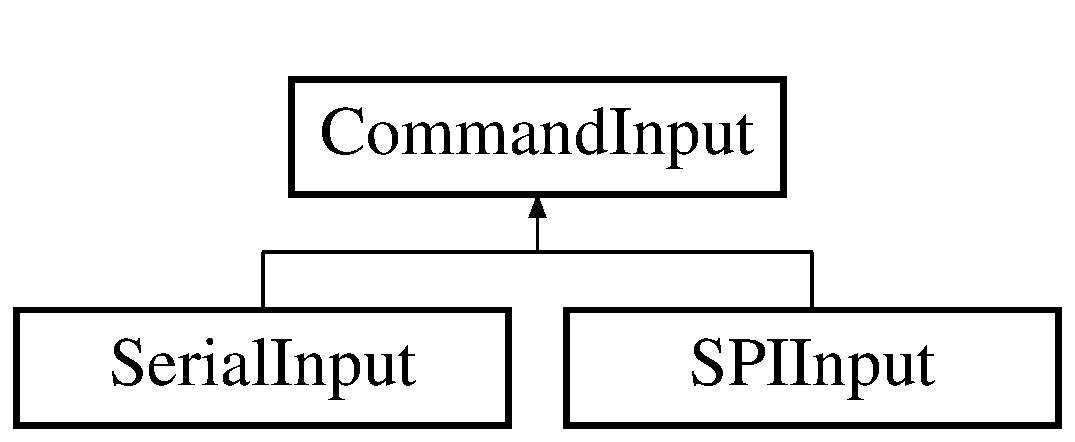
\includegraphics[height=2.000000cm]{classCommandInput}
\end{center}
\end{figure}
\subsection*{Public Member Functions}
\begin{DoxyCompactItemize}
\item 
\hypertarget{classCommandInput_adde08e78426afd0f6b8fd7274c08f289}{}virtual \hyperlink{classCommand}{Command} {\bfseries get\+Next\+Command} ()\label{classCommandInput_adde08e78426afd0f6b8fd7274c08f289}

\item 
\hypertarget{classCommandInput_a2d1a576856c671a36170fa27fe7d083c}{}virtual bool {\bfseries has\+Next\+Command} ()\label{classCommandInput_a2d1a576856c671a36170fa27fe7d083c}

\end{DoxyCompactItemize}


\subsection{Detailed Description}
Any source of commands. Could be through Bluetooth, Wifi, S\+P\+I, button pressing, etc... 

The documentation for this class was generated from the following files\+:\begin{DoxyCompactItemize}
\item 
src/\+Commands/\+Command\+Input/\hyperlink{CommandInput_8h}{Command\+Input.\+h}\item 
src/\+Commands/\+Command\+Input/\hyperlink{CommandInput_8cpp}{Command\+Input.\+cpp}\end{DoxyCompactItemize}

\hypertarget{classComponent}{}\section{Component Class Reference}
\label{classComponent}\index{Component@{Component}}


{\ttfamily \#include $<$Component.\+h$>$}

Inheritance diagram for Component\+:\begin{figure}[H]
\begin{center}
\leavevmode
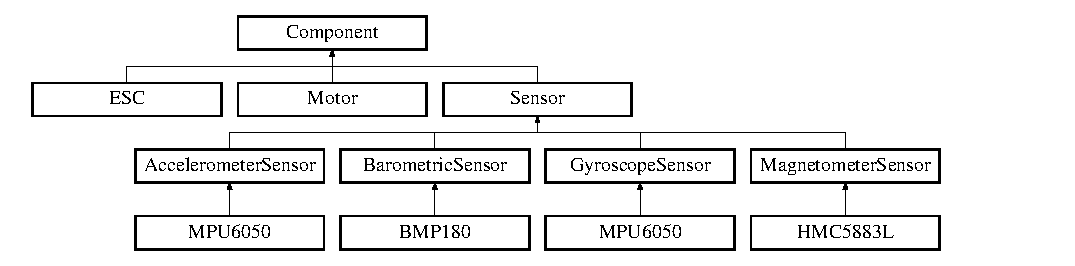
\includegraphics[height=3.132867cm]{classComponent}
\end{center}
\end{figure}
\subsection*{Public Member Functions}
\begin{DoxyCompactItemize}
\item 
\hyperlink{classComponent_a4a7922a1731595c86dce13e734967c12}{Component} (String name)
\item 
virtual \hyperlink{classComponent_ab8378fa275af98e568a7e91d33d867af}{$\sim$\+Component} ()
\item 
String \hyperlink{classComponent_a71a1eb698d3f6c69e900c9740a55ec95}{get\+Logging\+Info} ()
\end{DoxyCompactItemize}


\subsection{Detailed Description}
This virtual class represents every physical device used on the Multi\+Copter. 

\subsection{Constructor \& Destructor Documentation}
\hypertarget{classComponent_a4a7922a1731595c86dce13e734967c12}{}\index{Component@{Component}!Component@{Component}}
\index{Component@{Component}!Component@{Component}}
\subsubsection[{Component(\+String name)}]{\setlength{\rightskip}{0pt plus 5cm}Component\+::\+Component (
\begin{DoxyParamCaption}
\item[{String}]{name}
\end{DoxyParamCaption}
)}\label{classComponent_a4a7922a1731595c86dce13e734967c12}
Construct a new \hyperlink{classComponent}{Component} with the given name. \hypertarget{classComponent_ab8378fa275af98e568a7e91d33d867af}{}\index{Component@{Component}!````~Component@{$\sim$\+Component}}
\index{````~Component@{$\sim$\+Component}!Component@{Component}}
\subsubsection[{$\sim$\+Component()}]{\setlength{\rightskip}{0pt plus 5cm}Component\+::$\sim$\+Component (
\begin{DoxyParamCaption}
{}
\end{DoxyParamCaption}
)\hspace{0.3cm}{\ttfamily [virtual]}}\label{classComponent_ab8378fa275af98e568a7e91d33d867af}
Unused 

\subsection{Member Function Documentation}
\hypertarget{classComponent_a71a1eb698d3f6c69e900c9740a55ec95}{}\index{Component@{Component}!get\+Logging\+Info@{get\+Logging\+Info}}
\index{get\+Logging\+Info@{get\+Logging\+Info}!Component@{Component}}
\subsubsection[{get\+Logging\+Info()}]{\setlength{\rightskip}{0pt plus 5cm}String Component\+::get\+Logging\+Info (
\begin{DoxyParamCaption}
{}
\end{DoxyParamCaption}
)}\label{classComponent_a71a1eb698d3f6c69e900c9740a55ec95}
Return a non-\/newline ended string containing information about the \hyperlink{classComponent}{Component} 

The documentation for this class was generated from the following files\+:\begin{DoxyCompactItemize}
\item 
src/\+Components/\hyperlink{Component_8h}{Component.\+h}\item 
src/\+Components/\hyperlink{Component_8cpp}{Component.\+cpp}\end{DoxyCompactItemize}

\hypertarget{classESC}{}\section{E\+S\+C Class Reference}
\label{classESC}\index{E\+S\+C@{E\+S\+C}}


{\ttfamily \#include $<$E\+S\+C.\+h$>$}

Inheritance diagram for E\+S\+C\+:\begin{figure}[H]
\begin{center}
\leavevmode
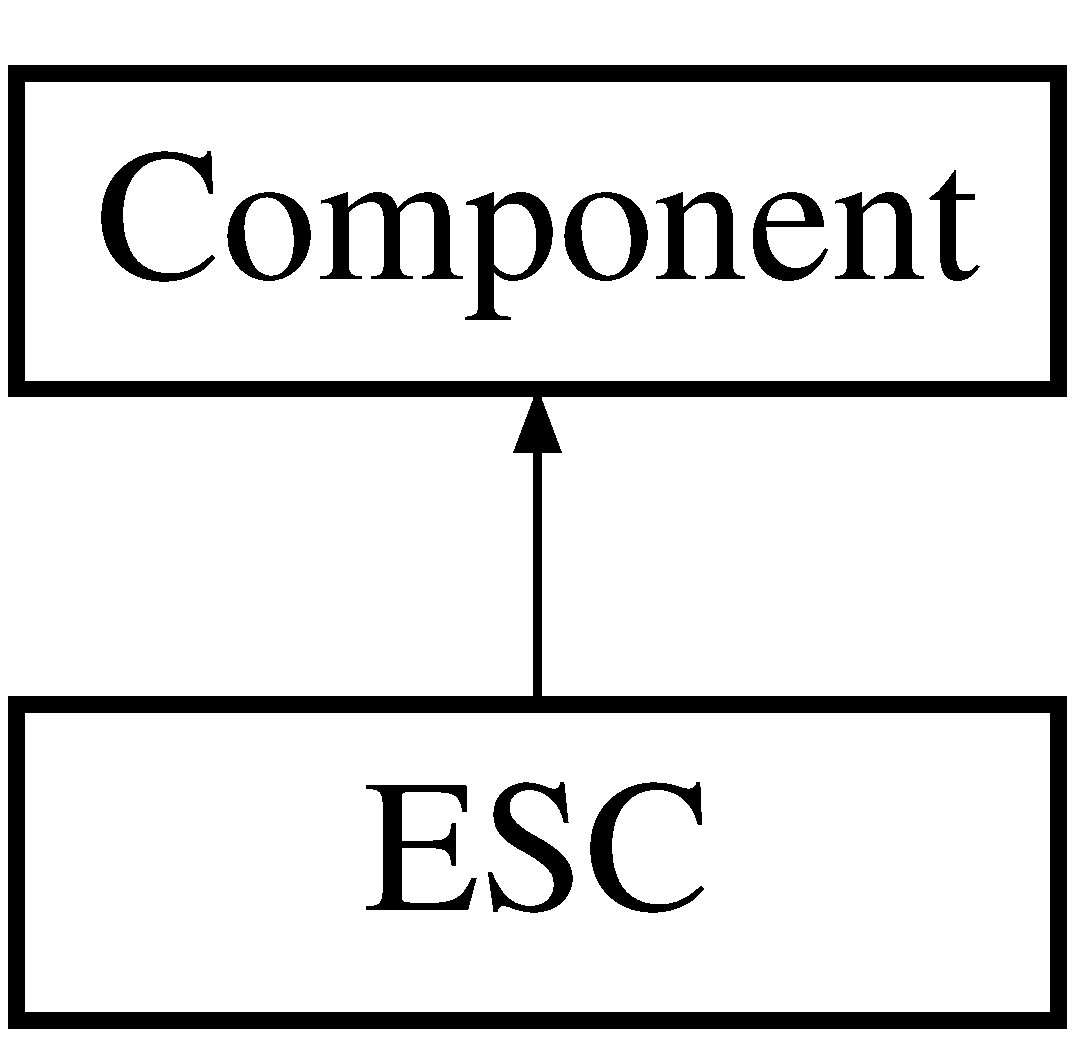
\includegraphics[height=2.000000cm]{classESC}
\end{center}
\end{figure}
\subsection*{Public Member Functions}
\begin{DoxyCompactItemize}
\item 
\hypertarget{classESC_a4254d339c64e305cb62ca42c6e439b9d}{}{\bfseries E\+S\+C} (String name, int pin, int position, \hyperlink{classMotor}{Motor} motor)\label{classESC_a4254d339c64e305cb62ca42c6e439b9d}

\item 
void \hyperlink{classESC_a4abfa0f0850c7c02c6e9c9adb405743d}{update\+Volatage} (float voltage)
\item 
\hypertarget{classESC_abdc82845ef1b09b94a89eba26610a8ff}{}String {\bfseries get\+Logging\+Info} ()\label{classESC_abdc82845ef1b09b94a89eba26610a8ff}

\end{DoxyCompactItemize}


\subsection{Detailed Description}
\hyperlink{classESC}{E\+S\+C} set voltage going to the motors. Basically, control where we are going. 
\begin{DoxyParams}{Parameters}
{\em pin} & what analog pin to write to \\
\hline
{\em position} & what position, clockwise from facing front, we are in. See picture somewhere... \\
\hline
\end{DoxyParams}


\subsection{Member Function Documentation}
\hypertarget{classESC_a4abfa0f0850c7c02c6e9c9adb405743d}{}\index{E\+S\+C@{E\+S\+C}!update\+Volatage@{update\+Volatage}}
\index{update\+Volatage@{update\+Volatage}!E\+S\+C@{E\+S\+C}}
\subsubsection[{update\+Volatage(float voltage)}]{\setlength{\rightskip}{0pt plus 5cm}void E\+S\+C\+::update\+Volatage (
\begin{DoxyParamCaption}
\item[{float}]{voltage}
\end{DoxyParamCaption}
)}\label{classESC_a4abfa0f0850c7c02c6e9c9adb405743d}
Updates the volatage for the \hyperlink{classESC}{E\+S\+C} 

The documentation for this class was generated from the following files\+:\begin{DoxyCompactItemize}
\item 
src/\+Components/\+E\+S\+C/\hyperlink{ESC_8h}{E\+S\+C.\+h}\item 
src/\+Components/\+E\+S\+C/\hyperlink{ESC_8cpp}{E\+S\+C.\+cpp}\end{DoxyCompactItemize}

\hypertarget{classESCConfig}{}\section{E\+S\+C\+Config Class Reference}
\label{classESCConfig}\index{E\+S\+C\+Config@{E\+S\+C\+Config}}
\subsection*{Public Member Functions}
\begin{DoxyCompactItemize}
\item 
\hypertarget{classESCConfig_a4fa17d962c059d2ea3fc3505893acbe1}{}{\bfseries E\+S\+C\+Config} (E\+S\+C\+L\+A\+Y\+O\+U\+T layout, \hyperlink{classESC}{E\+S\+C} e1, \hyperlink{classESC}{E\+S\+C} e2, \hyperlink{classESC}{E\+S\+C} e3, \hyperlink{classESC}{E\+S\+C} e4, \hyperlink{classESC}{E\+S\+C} e5, \hyperlink{classESC}{E\+S\+C} e6, \hyperlink{classESC}{E\+S\+C} e7, \hyperlink{classESC}{E\+S\+C} e8)\label{classESCConfig_a4fa17d962c059d2ea3fc3505893acbe1}

\item 
\hypertarget{classESCConfig_a4224f98b7b7b376cbb9623443a7759a5}{}bool {\bfseries validate\+Layout} ()\label{classESCConfig_a4224f98b7b7b376cbb9623443a7759a5}

\item 
\hypertarget{classESCConfig_a79c10721918440e631cca0fc754402ad}{}String {\bfseries get\+Logging\+Info} ()\label{classESCConfig_a79c10721918440e631cca0fc754402ad}

\end{DoxyCompactItemize}


The documentation for this class was generated from the following files\+:\begin{DoxyCompactItemize}
\item 
src/\+Components/\+E\+S\+C/\hyperlink{ESCConfig_8h}{E\+S\+C\+Config.\+h}\item 
src/\+Components/\+E\+S\+C/\hyperlink{ESCConfig_8cpp}{E\+S\+C\+Config.\+cpp}\end{DoxyCompactItemize}

\hypertarget{classFlightController}{}\section{Flight\+Controller Class Reference}
\label{classFlightController}\index{Flight\+Controller@{Flight\+Controller}}


{\ttfamily \#include $<$Flight\+Controller.\+h$>$}



\subsection{Detailed Description}
Flight Controller is composed of physical parts that enable it to fly. Flight controller decides when to read from each part. 

The documentation for this class was generated from the following files\+:\begin{DoxyCompactItemize}
\item 
src/\+Flight\+Controller/\hyperlink{FlightController_8h}{Flight\+Controller.\+h}\item 
src/\+Flight\+Controller/\hyperlink{FlightController_8cpp}{Flight\+Controller.\+cpp}\end{DoxyCompactItemize}

\hypertarget{classGPSStabilizer}{}\section{G\+P\+S\+Stabilizer Class Reference}
\label{classGPSStabilizer}\index{G\+P\+S\+Stabilizer@{G\+P\+S\+Stabilizer}}


The documentation for this class was generated from the following files\+:\begin{DoxyCompactItemize}
\item 
src/\+Flight\+Controller/\+Stabilizer/\+Stabilizers/G\+P\+S\+Stabilizer.\+h\item 
src/\+Flight\+Controller/\+Stabilizer/\+Stabilizers/G\+P\+S\+Stabilizer.\+cpp\end{DoxyCompactItemize}

\hypertarget{classGyroscopeSensor}{}\section{Gyroscope\+Sensor Class Reference}
\label{classGyroscopeSensor}\index{Gyroscope\+Sensor@{Gyroscope\+Sensor}}
Inheritance diagram for Gyroscope\+Sensor\+:\begin{figure}[H]
\begin{center}
\leavevmode
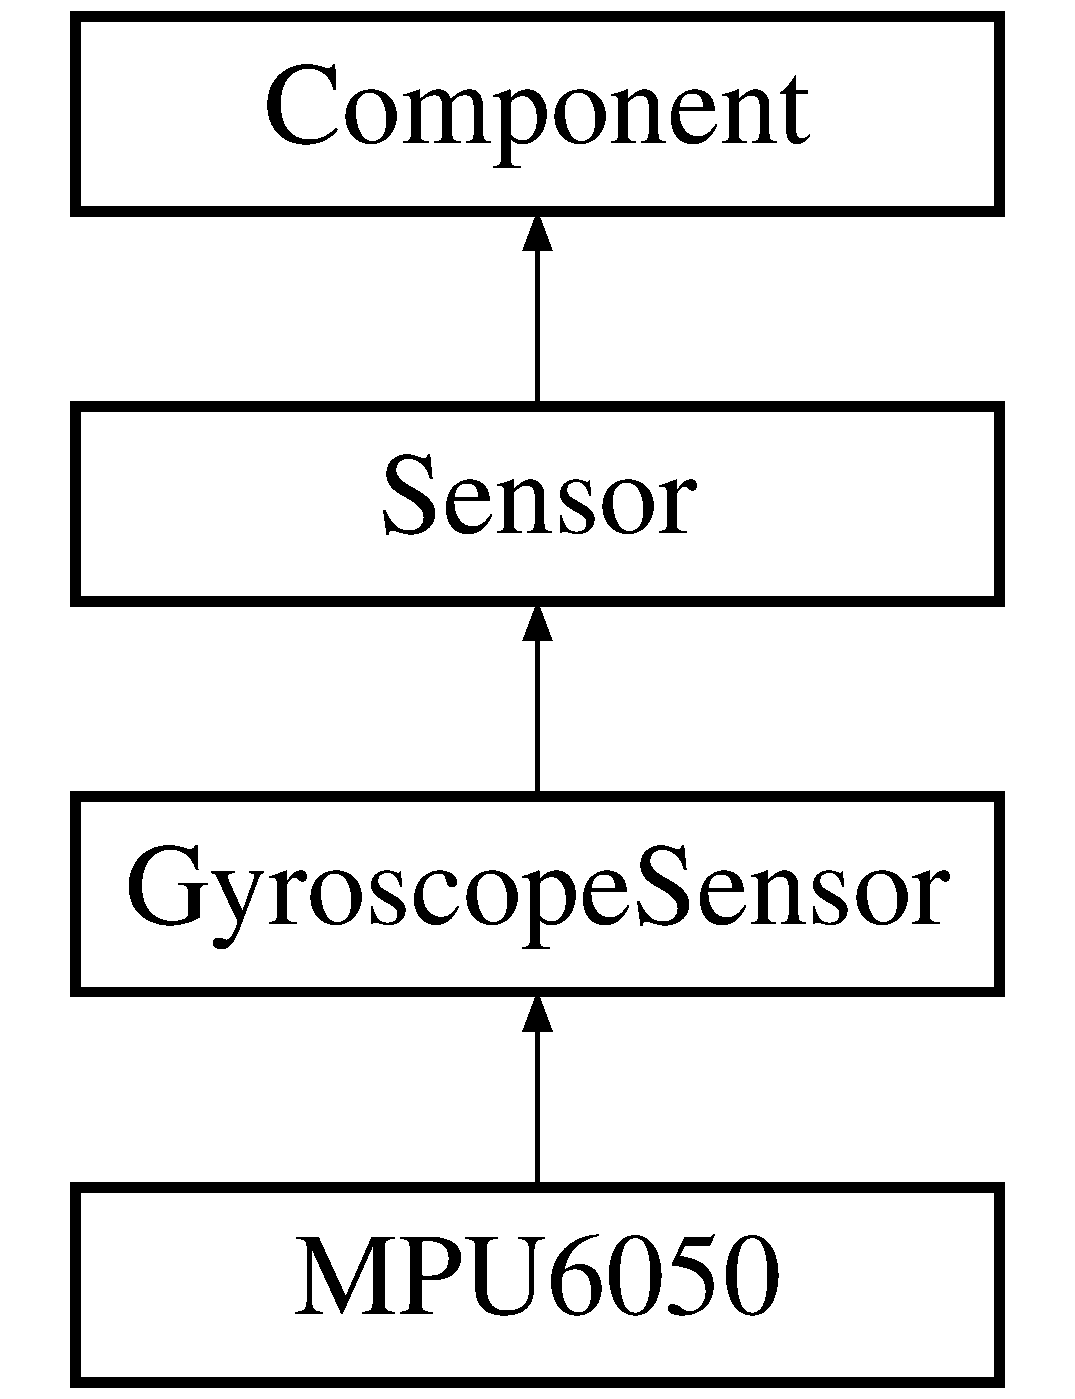
\includegraphics[height=4.000000cm]{classGyroscopeSensor}
\end{center}
\end{figure}
\subsection*{Public Member Functions}
\begin{DoxyCompactItemize}
\item 
\hypertarget{classGyroscopeSensor_a5e0f1b0f3aecb4078fca1067055c0a7b}{}{\bfseries Gyroscope\+Sensor} (String name)\label{classGyroscopeSensor_a5e0f1b0f3aecb4078fca1067055c0a7b}

\end{DoxyCompactItemize}


The documentation for this class was generated from the following files\+:\begin{DoxyCompactItemize}
\item 
src/\+Components/\+Sensor/\+Gyroscope\+Sensor/\hyperlink{GyroscopeSensor_8h}{Gyroscope\+Sensor.\+h}\item 
src/\+Components/\+Sensor/\+Gyroscope\+Sensor/\hyperlink{GyroscopeSensor_8cpp}{Gyroscope\+Sensor.\+cpp}\end{DoxyCompactItemize}

\hypertarget{classHMC5883L}{}\section{H\+M\+C5883\+L Class Reference}
\label{classHMC5883L}\index{H\+M\+C5883\+L@{H\+M\+C5883\+L}}
Inheritance diagram for H\+M\+C5883\+L\+:\begin{figure}[H]
\begin{center}
\leavevmode
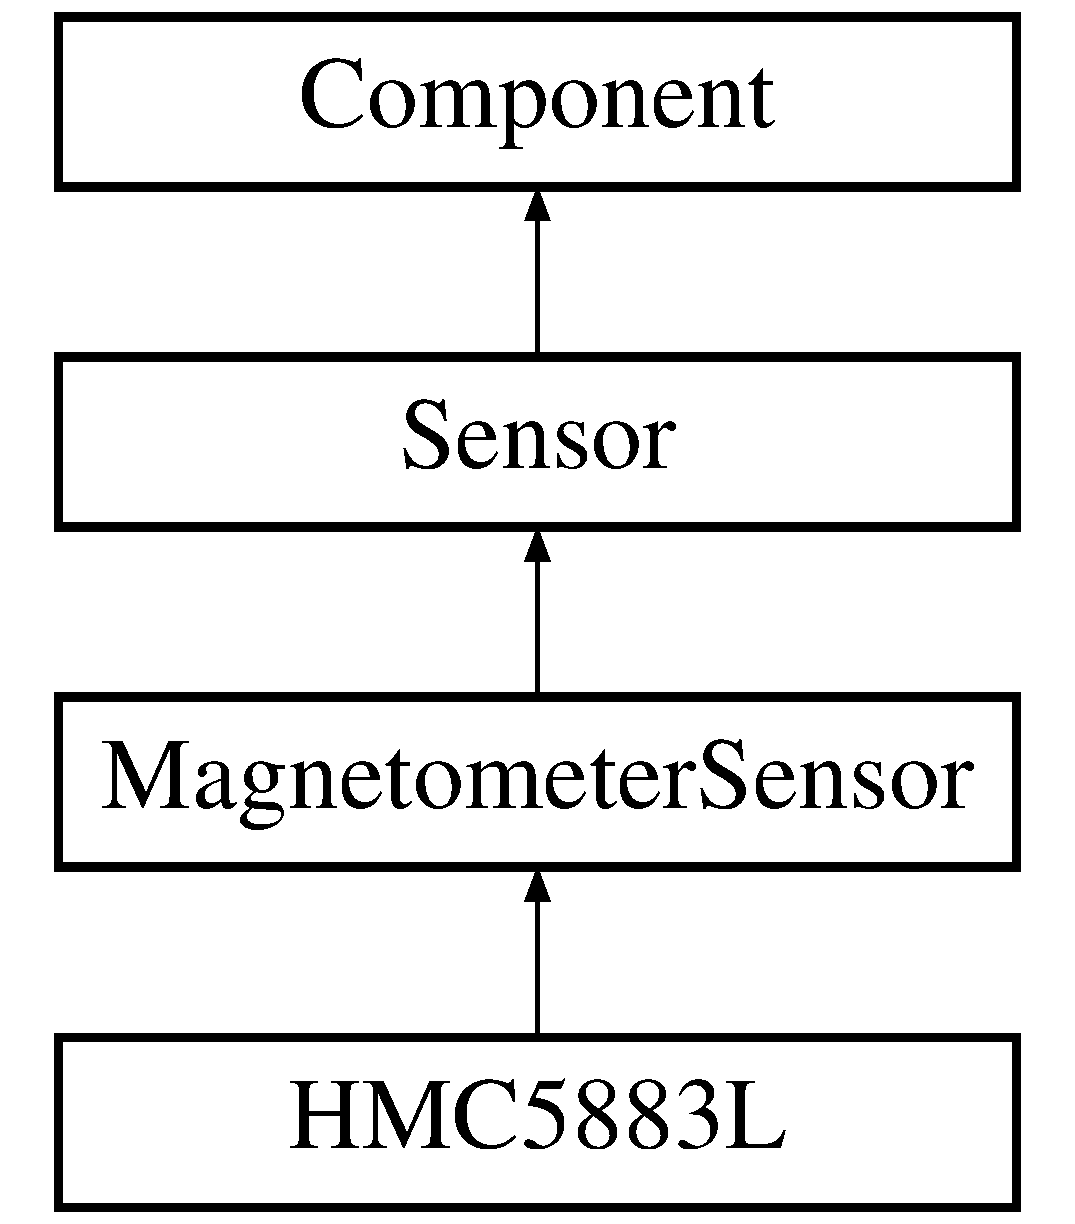
\includegraphics[height=4.000000cm]{classHMC5883L}
\end{center}
\end{figure}
\subsection*{Additional Inherited Members}


The documentation for this class was generated from the following files\+:\begin{DoxyCompactItemize}
\item 
src/\+Components/\+Parts/\+H\+M\+C5883\+L/\hyperlink{HMC5883L_8h}{H\+M\+C5883\+L.\+h}\item 
src/\+Components/\+Parts/\+H\+M\+C5883\+L/\hyperlink{HMC5883L_8cpp}{H\+M\+C5883\+L.\+cpp}\end{DoxyCompactItemize}

\hypertarget{classMagnetometerSensor}{}\section{Magnetometer\+Sensor Class Reference}
\label{classMagnetometerSensor}\index{Magnetometer\+Sensor@{Magnetometer\+Sensor}}
Inheritance diagram for Magnetometer\+Sensor\+:\begin{figure}[H]
\begin{center}
\leavevmode
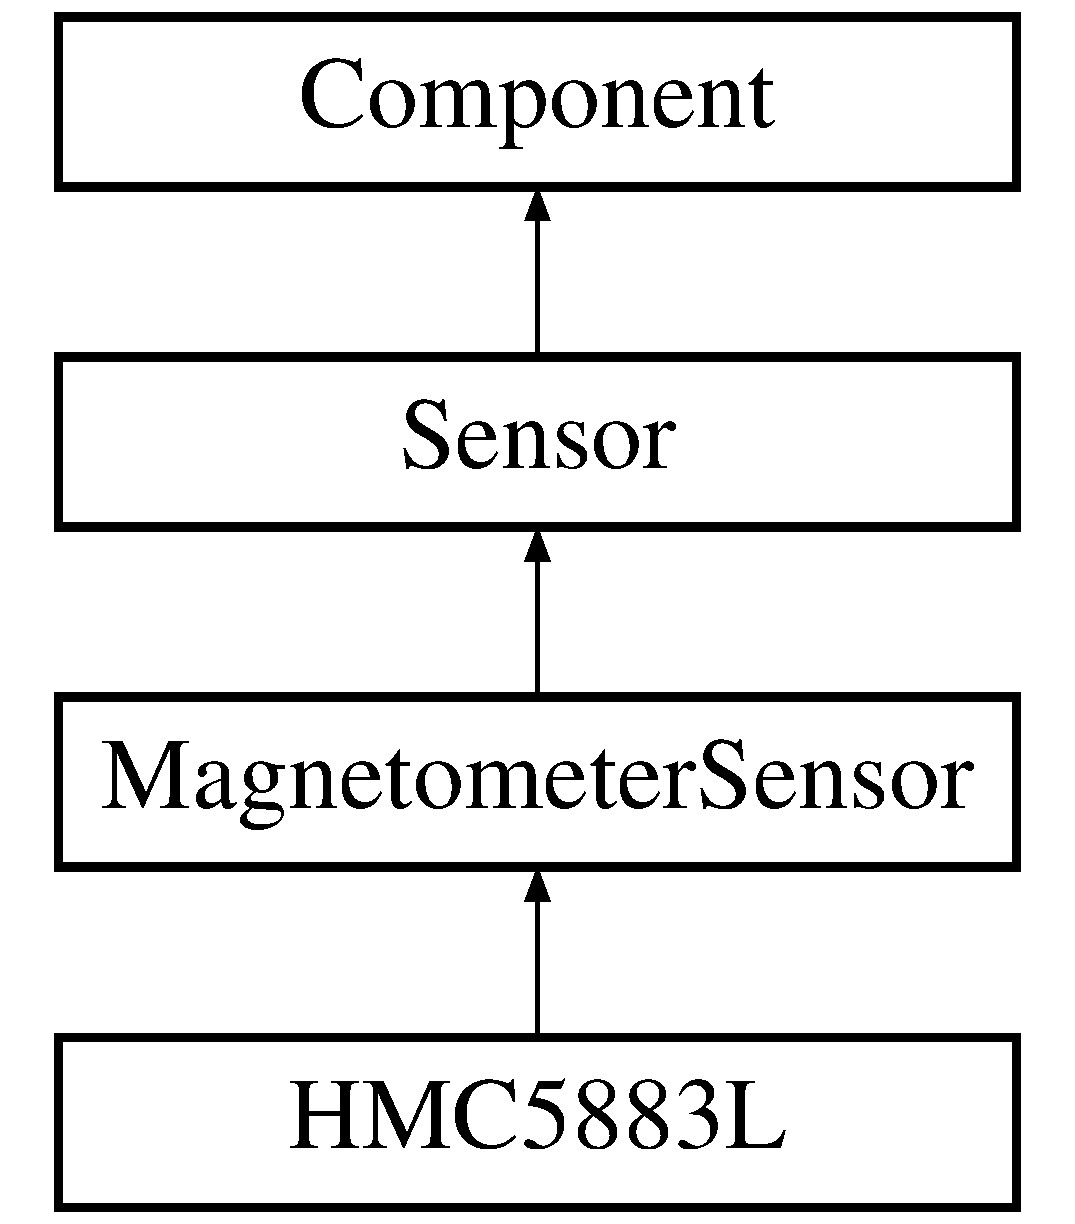
\includegraphics[height=4.000000cm]{classMagnetometerSensor}
\end{center}
\end{figure}
\subsection*{Public Member Functions}
\begin{DoxyCompactItemize}
\item 
\hypertarget{classMagnetometerSensor_a638465f24911a3a246e1e268f5159a2f}{}{\bfseries Magnetometer\+Sensor} (String name)\label{classMagnetometerSensor_a638465f24911a3a246e1e268f5159a2f}

\end{DoxyCompactItemize}


The documentation for this class was generated from the following files\+:\begin{DoxyCompactItemize}
\item 
src/\+Components/\+Sensor/\+Magnetometer\+Sensor/\hyperlink{MagnetometerSensor_8h}{Magnetometer\+Sensor.\+h}\item 
src/\+Components/\+Sensor/\+Magnetometer\+Sensor/\hyperlink{MagnetometerSensor_8cpp}{Magnetometer\+Sensor.\+cpp}\end{DoxyCompactItemize}

\hypertarget{classMotor}{}\section{Motor Class Reference}
\label{classMotor}\index{Motor@{Motor}}
Inheritance diagram for Motor\+:\begin{figure}[H]
\begin{center}
\leavevmode
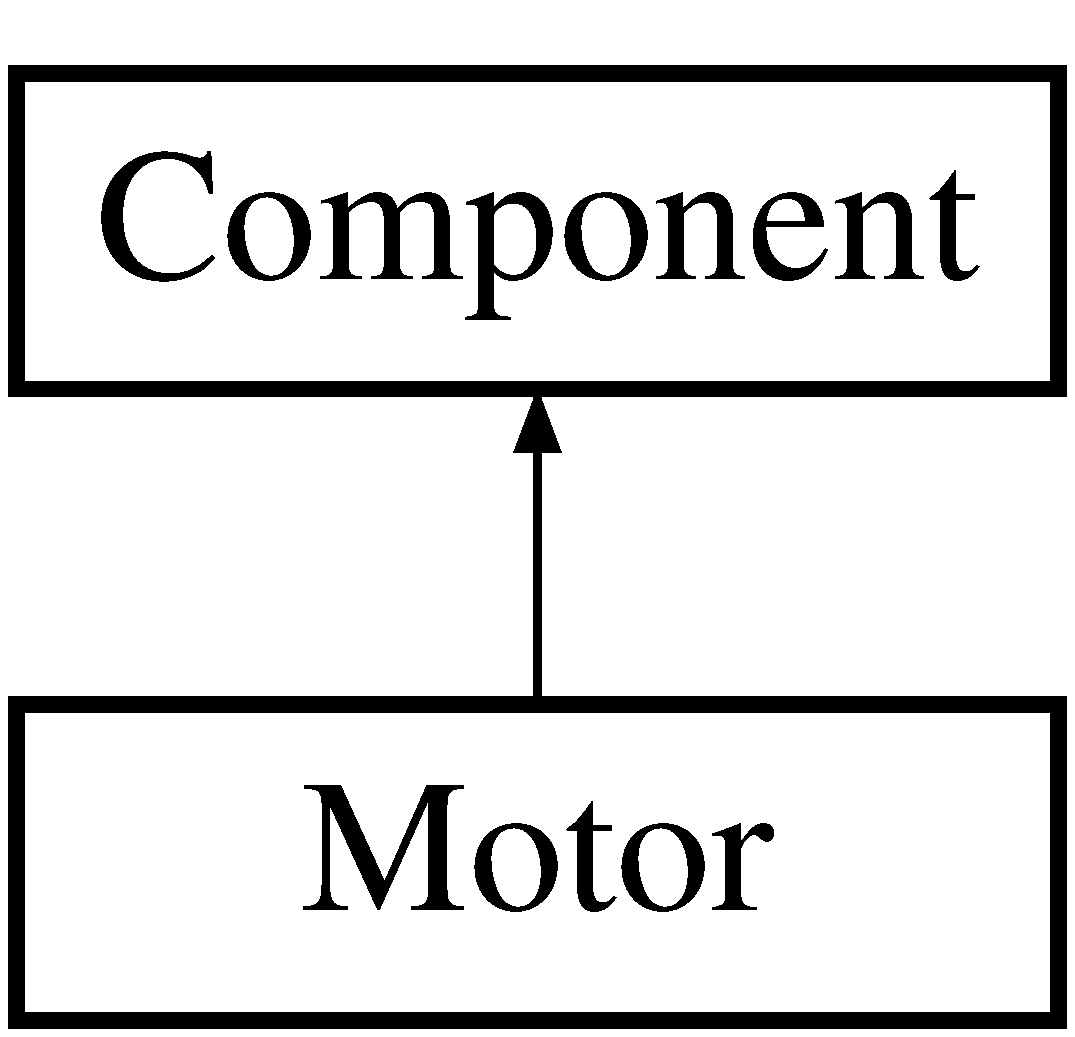
\includegraphics[height=2.000000cm]{classMotor}
\end{center}
\end{figure}
\subsection*{Public Member Functions}
\begin{DoxyCompactItemize}
\item 
\hyperlink{classMotor_ae46ff5cf1beb9197321e31fa406de083}{Motor} (const \hyperlink{classMotor}{Motor} \&motor)
\item 
\hyperlink{classMotor_af6106b4c506411265c5face762b6c004}{Motor} ()
\end{DoxyCompactItemize}


\subsection{Constructor \& Destructor Documentation}
\hypertarget{classMotor_ae46ff5cf1beb9197321e31fa406de083}{}\index{Motor@{Motor}!Motor@{Motor}}
\index{Motor@{Motor}!Motor@{Motor}}
\subsubsection[{Motor(const Motor \&motor)}]{\setlength{\rightskip}{0pt plus 5cm}Motor\+::\+Motor (
\begin{DoxyParamCaption}
\item[{const {\bf Motor} \&}]{motor}
\end{DoxyParamCaption}
)}\label{classMotor_ae46ff5cf1beb9197321e31fa406de083}
Create a \hyperlink{classMotor}{Motor} from another \hyperlink{classMotor}{Motor} \hypertarget{classMotor_af6106b4c506411265c5face762b6c004}{}\index{Motor@{Motor}!Motor@{Motor}}
\index{Motor@{Motor}!Motor@{Motor}}
\subsubsection[{Motor()}]{\setlength{\rightskip}{0pt plus 5cm}Motor\+::\+Motor (
\begin{DoxyParamCaption}
{}
\end{DoxyParamCaption}
)}\label{classMotor_af6106b4c506411265c5face762b6c004}
Construct a motor with the given name 

The documentation for this class was generated from the following files\+:\begin{DoxyCompactItemize}
\item 
src/\+Components/\+Motor/\hyperlink{Motor_8h}{Motor.\+h}\item 
src/\+Components/\+Motor/\hyperlink{Motor_8cpp}{Motor.\+cpp}\end{DoxyCompactItemize}

\hypertarget{classMPU6050}{}\section{M\+P\+U6050 Class Reference}
\label{classMPU6050}\index{M\+P\+U6050@{M\+P\+U6050}}
Inheritance diagram for M\+P\+U6050\+:\begin{figure}[H]
\begin{center}
\leavevmode
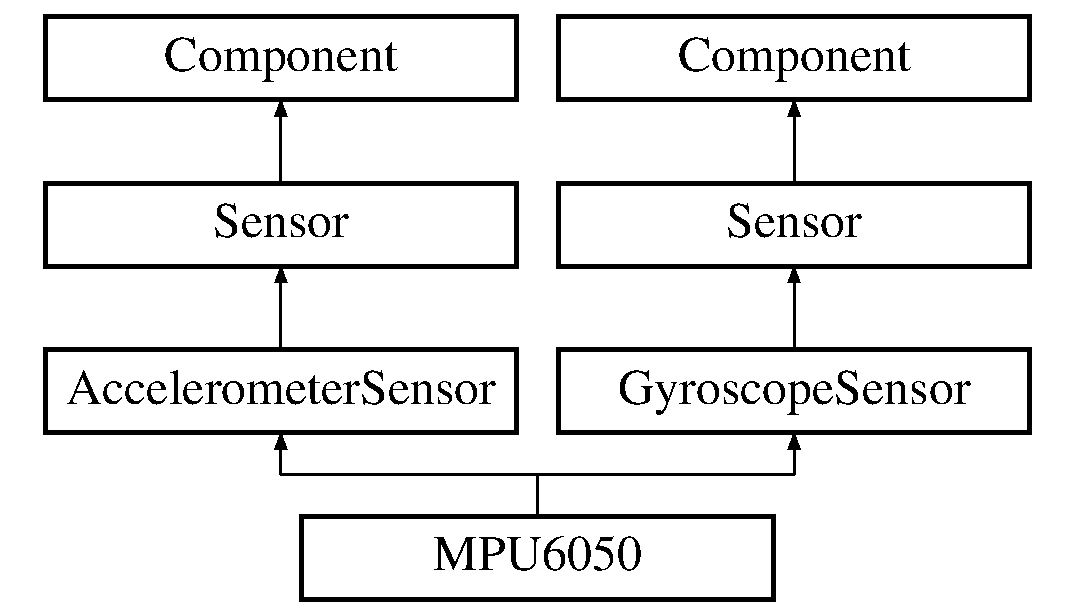
\includegraphics[height=4.000000cm]{classMPU6050}
\end{center}
\end{figure}
\subsection*{Additional Inherited Members}


The documentation for this class was generated from the following files\+:\begin{DoxyCompactItemize}
\item 
src/\+Components/\+Parts/\+M\+P\+U6050/\hyperlink{MPU6050_8h}{M\+P\+U6050.\+h}\item 
src/\+Components/\+Parts/\+M\+P\+U6050/\hyperlink{MPU6050_8cpp}{M\+P\+U6050.\+cpp}\end{DoxyCompactItemize}

\hypertarget{classPartsList}{}\section{Parts\+List Class Reference}
\label{classPartsList}\index{Parts\+List@{Parts\+List}}


{\ttfamily \#include $<$Parts\+List.\+h$>$}

\subsection*{Public Member Functions}
\begin{DoxyCompactItemize}
\item 
\hypertarget{classPartsList_a1c992c0e2ff567f6eae2997d25aeb469}{}{\bfseries Parts\+List} (const \hyperlink{classCommandInput}{Command\+Input} \&input, const \hyperlink{classESCConfig}{E\+S\+C\+Config} \&escconfig, const \hyperlink{classAccelerometerSensor}{Accelerometer\+Sensor} \&accelerometer\+Sensor, const \hyperlink{classGyroscopeSensor}{Gyroscope\+Sensor} \&gyroscope\+Sensor, const \hyperlink{classMagnetometerSensor}{Magnetometer\+Sensor} \&magnetometer\+Sensor)\label{classPartsList_a1c992c0e2ff567f6eae2997d25aeb469}

\end{DoxyCompactItemize}
\subsection*{Public Attributes}
\begin{DoxyCompactItemize}
\item 
\hypertarget{classPartsList_af7264b7c20a5ed198c75d6852e9e68a9}{}\hyperlink{classCommandInput}{Command\+Input} {\bfseries command\+Input}\label{classPartsList_af7264b7c20a5ed198c75d6852e9e68a9}

\item 
\hypertarget{classPartsList_a6138ab9e8359c557324a18f5f5849254}{}\hyperlink{classESCConfig}{E\+S\+C\+Config} {\bfseries esc\+Config}\label{classPartsList_a6138ab9e8359c557324a18f5f5849254}

\item 
\hypertarget{classPartsList_a2c7e98fdd3331ce7691197216789d9a6}{}\hyperlink{classAccelerometerSensor}{Accelerometer\+Sensor} {\bfseries accelerometer\+Sensor}\label{classPartsList_a2c7e98fdd3331ce7691197216789d9a6}

\item 
\hypertarget{classPartsList_a4111dff301073ea25c125b5d0778ad55}{}\hyperlink{classGyroscopeSensor}{Gyroscope\+Sensor} {\bfseries gyroscope\+Sensor}\label{classPartsList_a4111dff301073ea25c125b5d0778ad55}

\item 
\hypertarget{classPartsList_a9e344eccaec4f6410a1fc9028bcb0f37}{}\hyperlink{classMagnetometerSensor}{Magnetometer\+Sensor} {\bfseries magnetometer\+Sensor}\label{classPartsList_a9e344eccaec4f6410a1fc9028bcb0f37}

\end{DoxyCompactItemize}


\subsection{Detailed Description}
Used to neatly organize what is available on the Copter 

The documentation for this class was generated from the following files\+:\begin{DoxyCompactItemize}
\item 
src/\+Components/\+Parts/\hyperlink{PartsList_8h}{Parts\+List.\+h}\item 
src/\+Components/\+Parts/\hyperlink{PartsList_8cpp}{Parts\+List.\+cpp}\end{DoxyCompactItemize}

\hypertarget{classSensor}{}\section{Sensor Class Reference}
\label{classSensor}\index{Sensor@{Sensor}}


{\ttfamily \#include $<$Sensor.\+h$>$}

Inheritance diagram for Sensor\+:\begin{figure}[H]
\begin{center}
\leavevmode
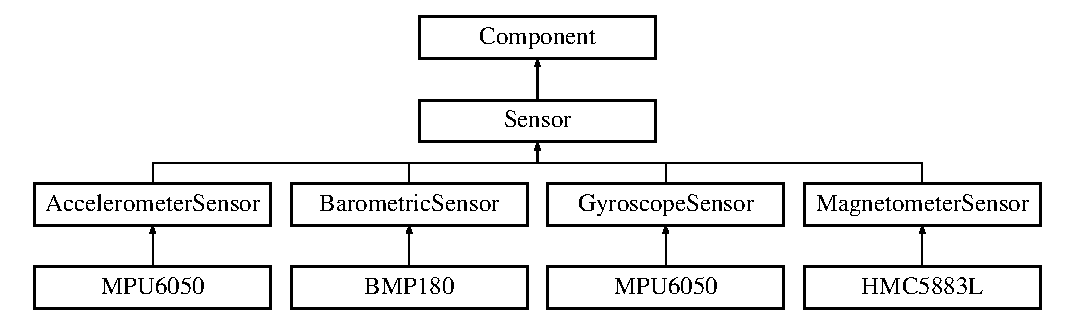
\includegraphics[height=3.916084cm]{classSensor}
\end{center}
\end{figure}
\subsection*{Public Member Functions}
\begin{DoxyCompactItemize}
\item 
\hyperlink{classSensor_a342d6d11ef572c8cba92cb76fb1a294b}{Sensor} ()
\item 
\hypertarget{classSensor_ad1e2c36720a75ee051925d062373a976}{}virtual void {\bfseries update\+Readings} ()\label{classSensor_ad1e2c36720a75ee051925d062373a976}

\end{DoxyCompactItemize}


\subsection{Detailed Description}
A \hyperlink{classSensor}{Sensor} is a \hyperlink{classComponent}{Component} that can gather information about anything. An example include a barometric sensor or a temperature sensor. A robot claw would N\+O\+T be a sensor. 

\subsection{Constructor \& Destructor Documentation}
\hypertarget{classSensor_a342d6d11ef572c8cba92cb76fb1a294b}{}\index{Sensor@{Sensor}!Sensor@{Sensor}}
\index{Sensor@{Sensor}!Sensor@{Sensor}}
\subsubsection[{Sensor()}]{\setlength{\rightskip}{0pt plus 5cm}Sensor\+::\+Sensor (
\begin{DoxyParamCaption}
{}
\end{DoxyParamCaption}
)}\label{classSensor_a342d6d11ef572c8cba92cb76fb1a294b}
Construct a new \hyperlink{classSensor}{Sensor} with the given name. 

The documentation for this class was generated from the following files\+:\begin{DoxyCompactItemize}
\item 
src/\+Components/\+Sensor/\hyperlink{Sensor_8h}{Sensor.\+h}\item 
src/\+Components/\+Sensor/\hyperlink{Sensor_8cpp}{Sensor.\+cpp}\end{DoxyCompactItemize}

\hypertarget{classSerialInput}{}\section{Serial\+Input Class Reference}
\label{classSerialInput}\index{Serial\+Input@{Serial\+Input}}
Inheritance diagram for Serial\+Input\+:\begin{figure}[H]
\begin{center}
\leavevmode
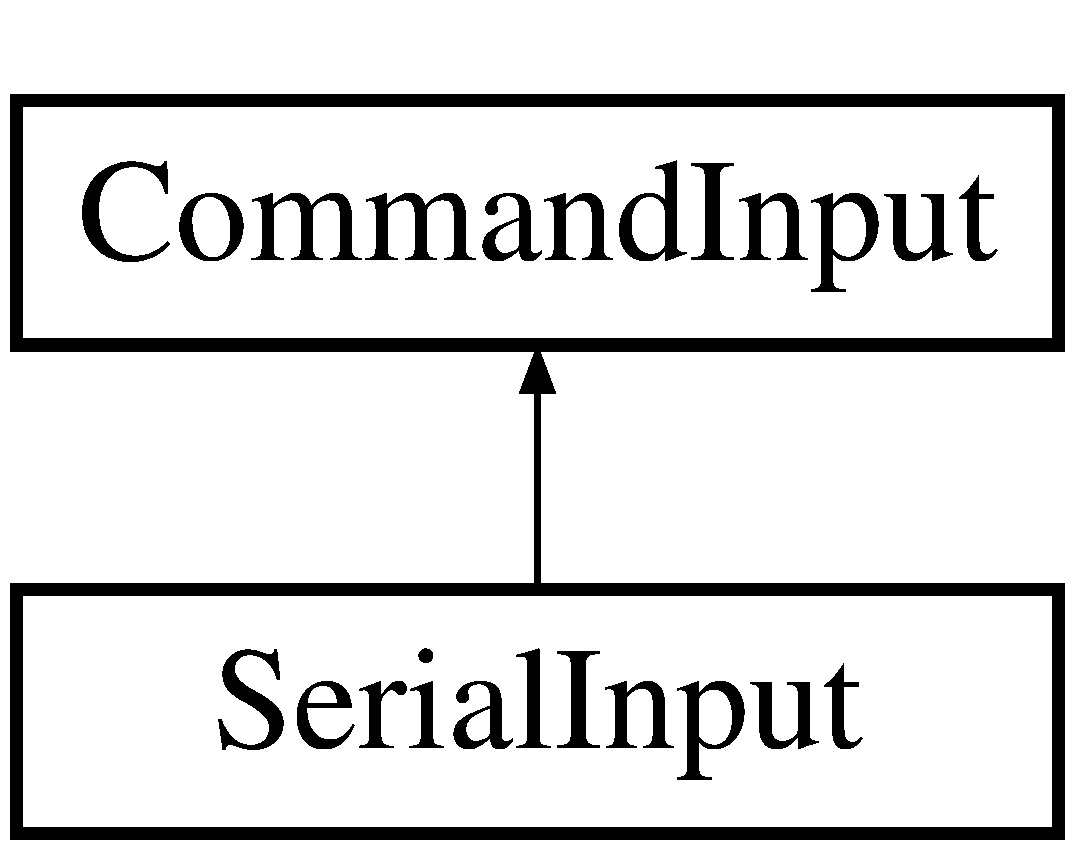
\includegraphics[height=2.000000cm]{classSerialInput}
\end{center}
\end{figure}
\subsection*{Public Member Functions}
\begin{DoxyCompactItemize}
\item 
\hypertarget{classSerialInput_a5e71f6970e190f77b5bbbeedabbefbc5}{}{\bfseries Serial\+Input} (int baud\+Rate)\label{classSerialInput_a5e71f6970e190f77b5bbbeedabbefbc5}

\item 
\hypertarget{classSerialInput_a9f4506bbeb54289553aab297d1fc7124}{}\hyperlink{classCommand}{Command} {\bfseries get\+Next\+Command} ()\label{classSerialInput_a9f4506bbeb54289553aab297d1fc7124}

\end{DoxyCompactItemize}


The documentation for this class was generated from the following files\+:\begin{DoxyCompactItemize}
\item 
src/\+Commands/\+Command\+Input/\+Inputs/\hyperlink{SerialInput_8h}{Serial\+Input.\+h}\item 
src/\+Commands/\+Command\+Input/\+Inputs/\hyperlink{SerialInput_8cpp}{Serial\+Input.\+cpp}\end{DoxyCompactItemize}

\hypertarget{classSPIInput}{}\section{S\+P\+I\+Input Class Reference}
\label{classSPIInput}\index{S\+P\+I\+Input@{S\+P\+I\+Input}}
Inheritance diagram for S\+P\+I\+Input\+:\begin{figure}[H]
\begin{center}
\leavevmode
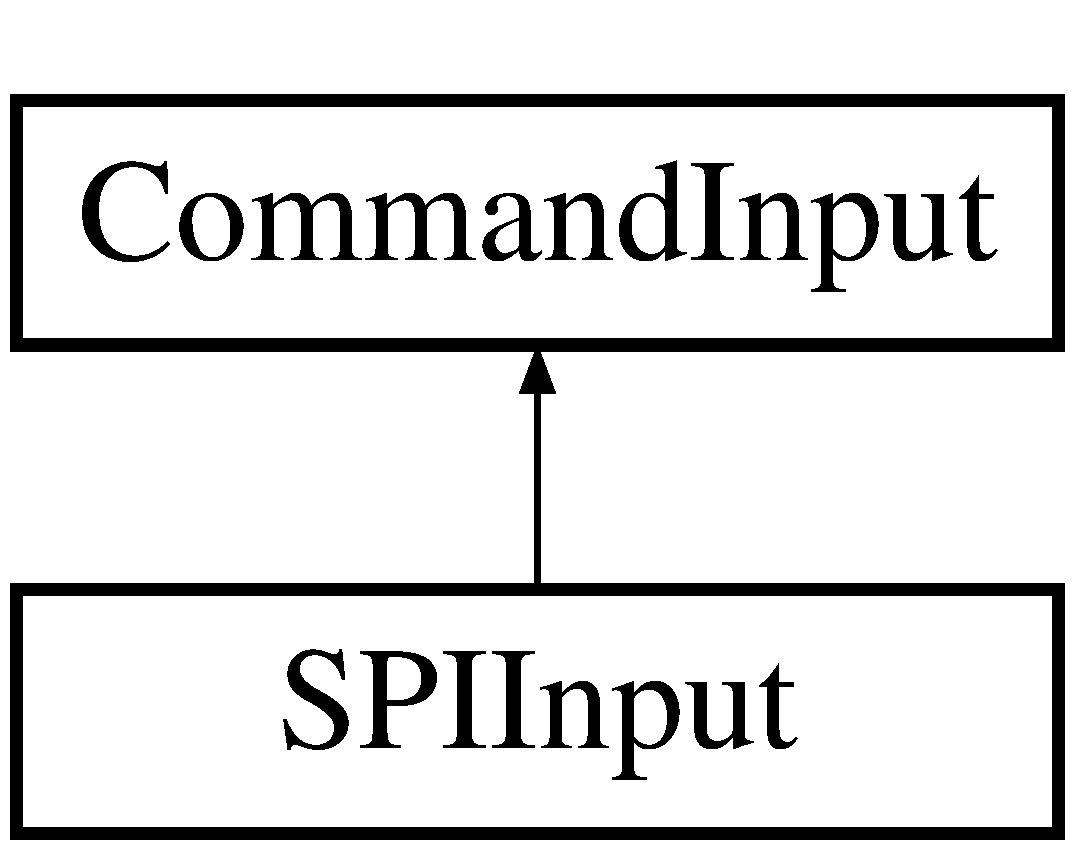
\includegraphics[height=2.000000cm]{classSPIInput}
\end{center}
\end{figure}
\subsection*{Additional Inherited Members}


The documentation for this class was generated from the following files\+:\begin{DoxyCompactItemize}
\item 
src/\+Commands/\+Command\+Input/\+Inputs/\hyperlink{SPIInput_8h}{S\+P\+I\+Input.\+h}\item 
src/\+Commands/\+Command\+Input/\+Inputs/\hyperlink{SPIInput_8cpp}{S\+P\+I\+Input.\+cpp}\end{DoxyCompactItemize}

\hypertarget{classStabilizer}{}\section{Stabilizer Class Reference}
\label{classStabilizer}\index{Stabilizer@{Stabilizer}}


The documentation for this class was generated from the following files\+:\begin{DoxyCompactItemize}
\item 
src/\+Flight\+Controller/\+Stabilizer/Stabilizer.\+h\item 
src/\+Flight\+Controller/\+Stabilizer/Stabilizer.\+cpp\end{DoxyCompactItemize}

\hypertarget{classUtil}{}\section{Util Class Reference}
\label{classUtil}\index{Util@{Util}}


The documentation for this class was generated from the following files\+:\begin{DoxyCompactItemize}
\item 
src/\+Util/\hyperlink{Util_8h}{Util.\+h}\item 
src/\+Util/\hyperlink{Util_8cpp}{Util.\+cpp}\end{DoxyCompactItemize}

\chapter{File Documentation}
\hypertarget{CommandInput_8cpp}{}\section{src/\+Commands/\+Command\+Input/\+Command\+Input.cpp File Reference}
\label{CommandInput_8cpp}\index{src/\+Commands/\+Command\+Input/\+Command\+Input.\+cpp@{src/\+Commands/\+Command\+Input/\+Command\+Input.\+cpp}}
{\ttfamily \#include \char`\"{}Command\+Input.\+h\char`\"{}}\\*


\subsection{Detailed Description}
\hyperlink{CommandInput_8cpp}{Command\+Input.\+cpp}

Created on\+: May 14, 2015 Author\+: user 
\hypertarget{CommandInput_8h}{}\section{src/\+Commands/\+Command\+Input/\+Command\+Input.h File Reference}
\label{CommandInput_8h}\index{src/\+Commands/\+Command\+Input/\+Command\+Input.\+h@{src/\+Commands/\+Command\+Input/\+Command\+Input.\+h}}
{\ttfamily \#include \char`\"{}Command.\+h\char`\"{}}\\*
\subsection*{Classes}
\begin{DoxyCompactItemize}
\item 
class \hyperlink{classCommandInput}{Command\+Input}
\end{DoxyCompactItemize}


\subsection{Detailed Description}
\hyperlink{CommandInput_8h}{Command\+Input.\+h}

Created on\+: May 14, 2015 Author\+: user 
\hypertarget{SerialInput_8cpp}{}\section{src/\+Commands/\+Command\+Input/\+Inputs/\+Serial\+Input.cpp File Reference}
\label{SerialInput_8cpp}\index{src/\+Commands/\+Command\+Input/\+Inputs/\+Serial\+Input.\+cpp@{src/\+Commands/\+Command\+Input/\+Inputs/\+Serial\+Input.\+cpp}}
{\ttfamily \#include \char`\"{}Serial\+Input.\+h\char`\"{}}\\*


\subsection{Detailed Description}
\hyperlink{SerialInput_8cpp}{Serial\+Input.\+cpp}

Created on\+: May 14, 2015 Author\+: user 
\hypertarget{SerialInput_8h}{}\section{src/\+Commands/\+Command\+Input/\+Inputs/\+Serial\+Input.h File Reference}
\label{SerialInput_8h}\index{src/\+Commands/\+Command\+Input/\+Inputs/\+Serial\+Input.\+h@{src/\+Commands/\+Command\+Input/\+Inputs/\+Serial\+Input.\+h}}
{\ttfamily \#include \char`\"{}Command\+Input.\+h\char`\"{}}\\*
\subsection*{Classes}
\begin{DoxyCompactItemize}
\item 
class \hyperlink{classSerialInput}{Serial\+Input}
\end{DoxyCompactItemize}


\subsection{Detailed Description}
\hyperlink{SerialInput_8h}{Serial\+Input.\+h}

Created on\+: May 14, 2015 Author\+: user 
\hypertarget{SPIInput_8cpp}{}\section{src/\+Commands/\+Command\+Input/\+Inputs/\+S\+P\+I\+Input.cpp File Reference}
\label{SPIInput_8cpp}\index{src/\+Commands/\+Command\+Input/\+Inputs/\+S\+P\+I\+Input.\+cpp@{src/\+Commands/\+Command\+Input/\+Inputs/\+S\+P\+I\+Input.\+cpp}}
{\ttfamily \#include \char`\"{}S\+P\+I\+Input.\+h\char`\"{}}\\*


\subsection{Detailed Description}
\hyperlink{SPIInput_8cpp}{S\+P\+I\+Input.\+cpp}

Created on\+: May 14, 2015 Author\+: user 
\hypertarget{SPIInput_8h}{}\section{src/\+Commands/\+Command\+Input/\+Inputs/\+S\+P\+I\+Input.h File Reference}
\label{SPIInput_8h}\index{src/\+Commands/\+Command\+Input/\+Inputs/\+S\+P\+I\+Input.\+h@{src/\+Commands/\+Command\+Input/\+Inputs/\+S\+P\+I\+Input.\+h}}
{\ttfamily \#include \char`\"{}Command\+Input.\+h\char`\"{}}\\*
\subsection*{Classes}
\begin{DoxyCompactItemize}
\item 
class \hyperlink{classSPIInput}{S\+P\+I\+Input}
\end{DoxyCompactItemize}


\subsection{Detailed Description}
\hyperlink{SPIInput_8h}{S\+P\+I\+Input.\+h}

Created on\+: May 14, 2015 Author\+: user 
\hypertarget{Protocol_8h}{}\section{src/\+Commands/\+Protocol.h File Reference}
\label{Protocol_8h}\index{src/\+Commands/\+Protocol.\+h@{src/\+Commands/\+Protocol.\+h}}
\subsection*{Enumerations}
\begin{DoxyCompactItemize}
\item 
enum \hyperlink{Protocol_8h_aa268a41a13430b18e933ed40207178d0}{D\+I\+R\+E\+C\+T\+I\+O\+N} \{ {\bfseries N\+O\+R\+T\+H}, 
{\bfseries E\+A\+S\+T}, 
{\bfseries S\+O\+U\+T\+H}, 
{\bfseries W\+E\+S\+T}
 \}
\item 
enum \hyperlink{Protocol_8h_a0fbada5bff0eeb4dc6be4b6e6f1c4eaf}{C\+O\+M\+M\+A\+N\+D} \{ \\*
{\bfseries N\+O\+N\+E}, 
{\bfseries I\+N\+T\+E\+R\+R\+U\+P\+T}, 
{\bfseries F\+O\+R\+W\+A\+R\+D}, 
{\bfseries B\+A\+C\+K\+W\+A\+R\+D}, 
\\*
{\bfseries L\+E\+F\+T}, 
{\bfseries R\+I\+G\+H\+T}, 
{\bfseries F\+L\+I\+P}, 
{\bfseries W\+A\+V\+E}
 \}
\end{DoxyCompactItemize}


\subsection{Detailed Description}
\hyperlink{Protocol_8h}{Protocol.\+h}

Created on\+: May 14, 2015 Author\+: user 

\subsection{Enumeration Type Documentation}
\hypertarget{Protocol_8h_a0fbada5bff0eeb4dc6be4b6e6f1c4eaf}{}\index{Protocol.\+h@{Protocol.\+h}!C\+O\+M\+M\+A\+N\+D@{C\+O\+M\+M\+A\+N\+D}}
\index{C\+O\+M\+M\+A\+N\+D@{C\+O\+M\+M\+A\+N\+D}!Protocol.\+h@{Protocol.\+h}}
\subsubsection[{C\+O\+M\+M\+A\+N\+D}]{\setlength{\rightskip}{0pt plus 5cm}enum {\bf C\+O\+M\+M\+A\+N\+D}}\label{Protocol_8h_a0fbada5bff0eeb4dc6be4b6e6f1c4eaf}
Possible commands. Might move to a more compact or predictable structure. \hypertarget{Protocol_8h_aa268a41a13430b18e933ed40207178d0}{}\index{Protocol.\+h@{Protocol.\+h}!D\+I\+R\+E\+C\+T\+I\+O\+N@{D\+I\+R\+E\+C\+T\+I\+O\+N}}
\index{D\+I\+R\+E\+C\+T\+I\+O\+N@{D\+I\+R\+E\+C\+T\+I\+O\+N}!Protocol.\+h@{Protocol.\+h}}
\subsubsection[{D\+I\+R\+E\+C\+T\+I\+O\+N}]{\setlength{\rightskip}{0pt plus 5cm}enum {\bf D\+I\+R\+E\+C\+T\+I\+O\+N}}\label{Protocol_8h_aa268a41a13430b18e933ed40207178d0}
Might be useful for something 
\hypertarget{Component_8cpp}{}\section{src/\+Components/\+Component.cpp File Reference}
\label{Component_8cpp}\index{src/\+Components/\+Component.\+cpp@{src/\+Components/\+Component.\+cpp}}
{\ttfamily \#include \char`\"{}Component.\+h\char`\"{}}\\*


\subsection{Detailed Description}
\hyperlink{Component_8cpp}{Component.\+cpp}

Created on\+: May 14, 2015 Author\+: user 
\hypertarget{Component_8h}{}\section{src/\+Components/\+Component.h File Reference}
\label{Component_8h}\index{src/\+Components/\+Component.\+h@{src/\+Components/\+Component.\+h}}
{\ttfamily \#include $<$W\+String.\+h$>$}\\*
\subsection*{Classes}
\begin{DoxyCompactItemize}
\item 
class \hyperlink{classComponent}{Component}
\end{DoxyCompactItemize}


\subsection{Detailed Description}
\hyperlink{Component_8h}{Component.\+h}

Created on\+: May 14, 2015 Author\+: user 
\hypertarget{ESC_8cpp}{}\section{src/\+Components/\+E\+S\+C/\+E\+S\+C.cpp File Reference}
\label{ESC_8cpp}\index{src/\+Components/\+E\+S\+C/\+E\+S\+C.\+cpp@{src/\+Components/\+E\+S\+C/\+E\+S\+C.\+cpp}}
{\ttfamily \#include \char`\"{}E\+S\+C.\+h\char`\"{}}\\*


\subsection{Detailed Description}
\hyperlink{ESC_8cpp}{E\+S\+C.\+cpp}

Created on\+: May 14, 2015 Author\+: user 
\hypertarget{ESC_8h}{}\section{src/\+Components/\+E\+S\+C/\+E\+S\+C.h File Reference}
\label{ESC_8h}\index{src/\+Components/\+E\+S\+C/\+E\+S\+C.\+h@{src/\+Components/\+E\+S\+C/\+E\+S\+C.\+h}}
{\ttfamily \#include \char`\"{}Motor.\+h\char`\"{}}\\*
\subsection*{Classes}
\begin{DoxyCompactItemize}
\item 
class \hyperlink{classESC}{E\+S\+C}
\end{DoxyCompactItemize}


\subsection{Detailed Description}
\hyperlink{ESC_8h}{E\+S\+C.\+h}

Created on\+: May 14, 2015 Author\+: user 
\hypertarget{ESCConfig_8cpp}{}\section{src/\+Components/\+E\+S\+C/\+E\+S\+C\+Config.cpp File Reference}
\label{ESCConfig_8cpp}\index{src/\+Components/\+E\+S\+C/\+E\+S\+C\+Config.\+cpp@{src/\+Components/\+E\+S\+C/\+E\+S\+C\+Config.\+cpp}}
{\ttfamily \#include \char`\"{}E\+S\+C\+Config.\+h\char`\"{}}\\*


\subsection{Detailed Description}
\hyperlink{ESCConfig_8cpp}{E\+S\+C\+Config.\+cpp}

Created on\+: May 14, 2015 Author\+: user 
\hypertarget{ESCConfig_8h}{}\section{src/\+Components/\+E\+S\+C/\+E\+S\+C\+Config.h File Reference}
\label{ESCConfig_8h}\index{src/\+Components/\+E\+S\+C/\+E\+S\+C\+Config.\+h@{src/\+Components/\+E\+S\+C/\+E\+S\+C\+Config.\+h}}
{\ttfamily \#include \char`\"{}E\+S\+C.\+h\char`\"{}}\\*
\subsection*{Classes}
\begin{DoxyCompactItemize}
\item 
class \hyperlink{classESCConfig}{E\+S\+C\+Config}
\end{DoxyCompactItemize}
\subsection*{Enumerations}
\begin{DoxyCompactItemize}
\item 
enum \hyperlink{ESCConfig_8h_a5e548692e60a92e800ad2e715a9f2303}{E\+S\+C\+L\+A\+Y\+O\+U\+T} \{ {\bfseries T\+R\+I}, 
{\bfseries Q\+U\+A\+D}, 
{\bfseries H\+E\+X\+A}, 
{\bfseries O\+C\+T\+A}
 \}
\end{DoxyCompactItemize}


\subsection{Detailed Description}
\hyperlink{ESCConfig_8h}{E\+S\+C\+Config.\+h}

Created on\+: May 14, 2015 Author\+: user 

\subsection{Enumeration Type Documentation}
\hypertarget{ESCConfig_8h_a5e548692e60a92e800ad2e715a9f2303}{}\index{E\+S\+C\+Config.\+h@{E\+S\+C\+Config.\+h}!E\+S\+C\+L\+A\+Y\+O\+U\+T@{E\+S\+C\+L\+A\+Y\+O\+U\+T}}
\index{E\+S\+C\+L\+A\+Y\+O\+U\+T@{E\+S\+C\+L\+A\+Y\+O\+U\+T}!E\+S\+C\+Config.\+h@{E\+S\+C\+Config.\+h}}
\subsubsection[{E\+S\+C\+L\+A\+Y\+O\+U\+T}]{\setlength{\rightskip}{0pt plus 5cm}enum {\bf E\+S\+C\+L\+A\+Y\+O\+U\+T}}\label{ESCConfig_8h_a5e548692e60a92e800ad2e715a9f2303}
Possible \hyperlink{classAutoCopter}{Auto\+Copter} layouts\+: Tri(3), Quad(4), Hexa(6), Octa(8) 
\hypertarget{Motor_8cpp}{}\section{src/\+Components/\+Motor/\+Motor.cpp File Reference}
\label{Motor_8cpp}\index{src/\+Components/\+Motor/\+Motor.\+cpp@{src/\+Components/\+Motor/\+Motor.\+cpp}}
{\ttfamily \#include $<$Motor/\+Motor.\+h$>$}\\*


\subsection{Detailed Description}
\hyperlink{Motor_8cpp}{Motor.\+cpp}

Created on\+: May 14, 2015 Author\+: user 
\hypertarget{Motor_8h}{}\section{src/\+Components/\+Motor/\+Motor.h File Reference}
\label{Motor_8h}\index{src/\+Components/\+Motor/\+Motor.\+h@{src/\+Components/\+Motor/\+Motor.\+h}}
{\ttfamily \#include \char`\"{}Component.\+h\char`\"{}}\\*
\subsection*{Classes}
\begin{DoxyCompactItemize}
\item 
class \hyperlink{classMotor}{Motor}
\end{DoxyCompactItemize}


\subsection{Detailed Description}
\hyperlink{Motor_8h}{Motor.\+h}

Created on\+: May 14, 2015 Author\+: user 
\hypertarget{BMP180_8cpp}{}\section{src/\+Components/\+Parts/\+B\+M\+P180/\+B\+M\+P180.cpp File Reference}
\label{BMP180_8cpp}\index{src/\+Components/\+Parts/\+B\+M\+P180/\+B\+M\+P180.\+cpp@{src/\+Components/\+Parts/\+B\+M\+P180/\+B\+M\+P180.\+cpp}}
{\ttfamily \#include \char`\"{}B\+M\+P180.\+h\char`\"{}}\\*


\subsection{Detailed Description}
\hyperlink{BMP180_8cpp}{B\+M\+P180.\+cpp}

Created on\+: May 14, 2015 Author\+: user 
\hypertarget{BMP180_8h}{}\section{src/\+Components/\+Parts/\+B\+M\+P180/\+B\+M\+P180.h File Reference}
\label{BMP180_8h}\index{src/\+Components/\+Parts/\+B\+M\+P180/\+B\+M\+P180.\+h@{src/\+Components/\+Parts/\+B\+M\+P180/\+B\+M\+P180.\+h}}
{\ttfamily \#include \char`\"{}Barometric\+Sensor.\+h\char`\"{}}\\*
\subsection*{Classes}
\begin{DoxyCompactItemize}
\item 
class \hyperlink{classBMP180}{B\+M\+P180}
\end{DoxyCompactItemize}


\subsection{Detailed Description}
\hyperlink{BMP180_8h}{B\+M\+P180.\+h}

Created on\+: May 14, 2015 Author\+: user 
\hypertarget{HMC5883L_8cpp}{}\section{src/\+Components/\+Parts/\+H\+M\+C5883\+L/\+H\+M\+C5883\+L.cpp File Reference}
\label{HMC5883L_8cpp}\index{src/\+Components/\+Parts/\+H\+M\+C5883\+L/\+H\+M\+C5883\+L.\+cpp@{src/\+Components/\+Parts/\+H\+M\+C5883\+L/\+H\+M\+C5883\+L.\+cpp}}
{\ttfamily \#include \char`\"{}H\+M\+C5883\+L.\+h\char`\"{}}\\*


\subsection{Detailed Description}
\hyperlink{HMC5883L_8cpp}{H\+M\+C5883\+L.\+cpp}

Created on\+: May 14, 2015 Author\+: user 
\hypertarget{HMC5883L_8h}{}\section{src/\+Components/\+Parts/\+H\+M\+C5883\+L/\+H\+M\+C5883\+L.h File Reference}
\label{HMC5883L_8h}\index{src/\+Components/\+Parts/\+H\+M\+C5883\+L/\+H\+M\+C5883\+L.\+h@{src/\+Components/\+Parts/\+H\+M\+C5883\+L/\+H\+M\+C5883\+L.\+h}}
{\ttfamily \#include \char`\"{}Magnetometer\+Sensor.\+h\char`\"{}}\\*
\subsection*{Classes}
\begin{DoxyCompactItemize}
\item 
class \hyperlink{classHMC5883L}{H\+M\+C5883\+L}
\end{DoxyCompactItemize}


\subsection{Detailed Description}
\hyperlink{HMC5883L_8h}{H\+M\+C5883\+L.\+h}

Created on\+: May 14, 2015 Author\+: user 
\hypertarget{MPU6050_8cpp}{}\section{src/\+Components/\+Parts/\+M\+P\+U6050/\+M\+P\+U6050.cpp File Reference}
\label{MPU6050_8cpp}\index{src/\+Components/\+Parts/\+M\+P\+U6050/\+M\+P\+U6050.\+cpp@{src/\+Components/\+Parts/\+M\+P\+U6050/\+M\+P\+U6050.\+cpp}}
{\ttfamily \#include $<$Parts/\+M\+P\+U6050/\+M\+P\+U6050.\+h$>$}\\*


\subsection{Detailed Description}
\hyperlink{MPU6050_8cpp}{M\+P\+U6050.\+cpp}

Created on\+: May 14, 2015 Author\+: user 
\hypertarget{MPU6050_8h}{}\section{src/\+Components/\+Parts/\+M\+P\+U6050/\+M\+P\+U6050.h File Reference}
\label{MPU6050_8h}\index{src/\+Components/\+Parts/\+M\+P\+U6050/\+M\+P\+U6050.\+h@{src/\+Components/\+Parts/\+M\+P\+U6050/\+M\+P\+U6050.\+h}}
{\ttfamily \#include \char`\"{}Accelerometer\+Sensor.\+h\char`\"{}}\\*
{\ttfamily \#include \char`\"{}Gyroscope\+Sensor.\+h\char`\"{}}\\*
\subsection*{Classes}
\begin{DoxyCompactItemize}
\item 
class \hyperlink{classMPU6050}{M\+P\+U6050}
\end{DoxyCompactItemize}


\subsection{Detailed Description}
\hyperlink{MPU6050_8h}{M\+P\+U6050.\+h}

Created on\+: May 14, 2015 Author\+: user 
\hypertarget{PartsList_8cpp}{}\section{src/\+Components/\+Parts/\+Parts\+List.cpp File Reference}
\label{PartsList_8cpp}\index{src/\+Components/\+Parts/\+Parts\+List.\+cpp@{src/\+Components/\+Parts/\+Parts\+List.\+cpp}}
{\ttfamily \#include \char`\"{}Parts\+List.\+h\char`\"{}}\\*


\subsection{Detailed Description}
\hyperlink{PartsList_8cpp}{Parts\+List.\+cpp}

Created on\+: May 14, 2015 Author\+: user 
\hypertarget{PartsList_8h}{}\section{src/\+Components/\+Parts/\+Parts\+List.h File Reference}
\label{PartsList_8h}\index{src/\+Components/\+Parts/\+Parts\+List.\+h@{src/\+Components/\+Parts/\+Parts\+List.\+h}}
{\ttfamily \#include \char`\"{}Command\+Input.\+h\char`\"{}}\\*
{\ttfamily \#include \char`\"{}E\+S\+C\+Config.\+h\char`\"{}}\\*
\subsection*{Classes}
\begin{DoxyCompactItemize}
\item 
class \hyperlink{classPartsList}{Parts\+List}
\end{DoxyCompactItemize}


\subsection{Detailed Description}
\hyperlink{PartsList_8h}{Parts\+List.\+h}

Created on\+: May 14, 2015 Author\+: user 
\hypertarget{AccelerometerSensor_8cpp}{}\section{src/\+Components/\+Sensor/\+Accelerometer\+Sensor/\+Accelerometer\+Sensor.cpp File Reference}
\label{AccelerometerSensor_8cpp}\index{src/\+Components/\+Sensor/\+Accelerometer\+Sensor/\+Accelerometer\+Sensor.\+cpp@{src/\+Components/\+Sensor/\+Accelerometer\+Sensor/\+Accelerometer\+Sensor.\+cpp}}
{\ttfamily \#include \char`\"{}Accelerometer\+Sensor.\+h\char`\"{}}\\*


\subsection{Detailed Description}
\hyperlink{AccelerometerSensor_8cpp}{Accelerometer\+Sensor.\+cpp}

Created on\+: May 14, 2015 Author\+: user 
\hypertarget{AccelerometerSensor_8h}{}\section{src/\+Components/\+Sensor/\+Accelerometer\+Sensor/\+Accelerometer\+Sensor.h File Reference}
\label{AccelerometerSensor_8h}\index{src/\+Components/\+Sensor/\+Accelerometer\+Sensor/\+Accelerometer\+Sensor.\+h@{src/\+Components/\+Sensor/\+Accelerometer\+Sensor/\+Accelerometer\+Sensor.\+h}}
{\ttfamily \#include \char`\"{}Sensor.\+h\char`\"{}}\\*
\subsection*{Classes}
\begin{DoxyCompactItemize}
\item 
class \hyperlink{classAccelerometerSensor}{Accelerometer\+Sensor}
\end{DoxyCompactItemize}


\subsection{Detailed Description}
\hyperlink{AccelerometerSensor_8h}{Accelerometer\+Sensor.\+h}

Created on\+: May 14, 2015 Author\+: user 
\hypertarget{BarometricSensor_8cpp}{}\section{src/\+Components/\+Sensor/\+Barometer\+Sensor/\+Barometric\+Sensor.cpp File Reference}
\label{BarometricSensor_8cpp}\index{src/\+Components/\+Sensor/\+Barometer\+Sensor/\+Barometric\+Sensor.\+cpp@{src/\+Components/\+Sensor/\+Barometer\+Sensor/\+Barometric\+Sensor.\+cpp}}
{\ttfamily \#include \char`\"{}Barometric\+Sensor.\+h\char`\"{}}\\*


\subsection{Detailed Description}
\hyperlink{BarometricSensor_8cpp}{Barometric\+Sensor.\+cpp}

Created on\+: May 14, 2015 Author\+: user 
\hypertarget{BarometricSensor_8h}{}\section{src/\+Components/\+Sensor/\+Barometer\+Sensor/\+Barometric\+Sensor.h File Reference}
\label{BarometricSensor_8h}\index{src/\+Components/\+Sensor/\+Barometer\+Sensor/\+Barometric\+Sensor.\+h@{src/\+Components/\+Sensor/\+Barometer\+Sensor/\+Barometric\+Sensor.\+h}}
{\ttfamily \#include \char`\"{}Sensor.\+h\char`\"{}}\\*
\subsection*{Classes}
\begin{DoxyCompactItemize}
\item 
class \hyperlink{classBarometricSensor}{Barometric\+Sensor}
\end{DoxyCompactItemize}


\subsection{Detailed Description}
\hyperlink{BarometricSensor_8h}{Barometric\+Sensor.\+h}

Created on\+: May 14, 2015 Author\+: user 
\hypertarget{GyroscopeSensor_8cpp}{}\section{src/\+Components/\+Sensor/\+Gyroscope\+Sensor/\+Gyroscope\+Sensor.cpp File Reference}
\label{GyroscopeSensor_8cpp}\index{src/\+Components/\+Sensor/\+Gyroscope\+Sensor/\+Gyroscope\+Sensor.\+cpp@{src/\+Components/\+Sensor/\+Gyroscope\+Sensor/\+Gyroscope\+Sensor.\+cpp}}
{\ttfamily \#include \char`\"{}Gyroscope\+Sensor.\+h\char`\"{}}\\*


\subsection{Detailed Description}
\hyperlink{GyroscopeSensor_8cpp}{Gyroscope\+Sensor.\+cpp}

Created on\+: May 14, 2015 Author\+: user 
\hypertarget{GyroscopeSensor_8h}{}\section{src/\+Components/\+Sensor/\+Gyroscope\+Sensor/\+Gyroscope\+Sensor.h File Reference}
\label{GyroscopeSensor_8h}\index{src/\+Components/\+Sensor/\+Gyroscope\+Sensor/\+Gyroscope\+Sensor.\+h@{src/\+Components/\+Sensor/\+Gyroscope\+Sensor/\+Gyroscope\+Sensor.\+h}}
{\ttfamily \#include \char`\"{}Sensor.\+h\char`\"{}}\\*
\subsection*{Classes}
\begin{DoxyCompactItemize}
\item 
class \hyperlink{classGyroscopeSensor}{Gyroscope\+Sensor}
\end{DoxyCompactItemize}


\subsection{Detailed Description}
\hyperlink{GyroscopeSensor_8h}{Gyroscope\+Sensor.\+h}

Created on\+: May 14, 2015 Author\+: user 
\hypertarget{MagnetometerSensor_8cpp}{}\section{src/\+Components/\+Sensor/\+Magnetometer\+Sensor/\+Magnetometer\+Sensor.cpp File Reference}
\label{MagnetometerSensor_8cpp}\index{src/\+Components/\+Sensor/\+Magnetometer\+Sensor/\+Magnetometer\+Sensor.\+cpp@{src/\+Components/\+Sensor/\+Magnetometer\+Sensor/\+Magnetometer\+Sensor.\+cpp}}
{\ttfamily \#include $<$Magnetometer\+Sensor/\+Magnetometer\+Sensor.\+h$>$}\\*


\subsection{Detailed Description}
\hyperlink{MagnetometerSensor_8cpp}{Magnetometer\+Sensor.\+cpp}

Created on\+: May 14, 2015 Author\+: user 
\hypertarget{MagnetometerSensor_8h}{}\section{src/\+Components/\+Sensor/\+Magnetometer\+Sensor/\+Magnetometer\+Sensor.h File Reference}
\label{MagnetometerSensor_8h}\index{src/\+Components/\+Sensor/\+Magnetometer\+Sensor/\+Magnetometer\+Sensor.\+h@{src/\+Components/\+Sensor/\+Magnetometer\+Sensor/\+Magnetometer\+Sensor.\+h}}
{\ttfamily \#include \char`\"{}Sensor.\+h\char`\"{}}\\*
\subsection*{Classes}
\begin{DoxyCompactItemize}
\item 
class \hyperlink{classMagnetometerSensor}{Magnetometer\+Sensor}
\end{DoxyCompactItemize}


\subsection{Detailed Description}
\hyperlink{MagnetometerSensor_8h}{Magnetometer\+Sensor.\+h}

Created on\+: May 14, 2015 Author\+: user 
\hypertarget{Sensor_8cpp}{}\section{src/\+Components/\+Sensor/\+Sensor.cpp File Reference}
\label{Sensor_8cpp}\index{src/\+Components/\+Sensor/\+Sensor.\+cpp@{src/\+Components/\+Sensor/\+Sensor.\+cpp}}
{\ttfamily \#include \char`\"{}Sensor.\+h\char`\"{}}\\*


\subsection{Detailed Description}
\hyperlink{Sensor_8cpp}{Sensor.\+cpp}

Created on\+: May 14, 2015 Author\+: user 
\hypertarget{Sensor_8h}{}\section{src/\+Components/\+Sensor/\+Sensor.h File Reference}
\label{Sensor_8h}\index{src/\+Components/\+Sensor/\+Sensor.\+h@{src/\+Components/\+Sensor/\+Sensor.\+h}}
{\ttfamily \#include \char`\"{}Component.\+h\char`\"{}}\\*
\subsection*{Classes}
\begin{DoxyCompactItemize}
\item 
class \hyperlink{classSensor}{Sensor}
\end{DoxyCompactItemize}


\subsection{Detailed Description}
\hyperlink{Sensor_8h}{Sensor.\+h}

Created on\+: May 14, 2015 Author\+: user 
\hypertarget{FlightController_8cpp}{}\section{src/\+Flight\+Controller/\+Flight\+Controller.cpp File Reference}
\label{FlightController_8cpp}\index{src/\+Flight\+Controller/\+Flight\+Controller.\+cpp@{src/\+Flight\+Controller/\+Flight\+Controller.\+cpp}}
{\ttfamily \#include \char`\"{}Flight\+Controller.\+h\char`\"{}}\\*


\subsection{Detailed Description}
\hyperlink{FlightController_8cpp}{Flight\+Controller.\+cpp}

Created on\+: May 14, 2015 Author\+: user 
\hypertarget{FlightController_8h}{}\section{src/\+Flight\+Controller/\+Flight\+Controller.h File Reference}
\label{FlightController_8h}\index{src/\+Flight\+Controller/\+Flight\+Controller.\+h@{src/\+Flight\+Controller/\+Flight\+Controller.\+h}}
\subsection*{Classes}
\begin{DoxyCompactItemize}
\item 
class \hyperlink{classFlightController}{Flight\+Controller}
\end{DoxyCompactItemize}


\subsection{Detailed Description}
\hyperlink{FlightController_8h}{Flight\+Controller.\+h}

Created on\+: May 14, 2015 Author\+: user 
\hypertarget{AutoCopter_8cpp}{}\section{src/\+Main/\+Auto\+Copter.cpp File Reference}
\label{AutoCopter_8cpp}\index{src/\+Main/\+Auto\+Copter.\+cpp@{src/\+Main/\+Auto\+Copter.\+cpp}}
{\ttfamily \#include \char`\"{}Auto\+Copter.\+h\char`\"{}}\\*
{\ttfamily \#include $<$Hardware\+Serial.\+h$>$}\\*


\subsection{Detailed Description}
\hyperlink{AutoCopter_8cpp}{Auto\+Copter.\+cpp}

Created on\+: May 14, 2015 Author\+: user 
\hypertarget{AutoCopter_8h}{}\section{src/\+Main/\+Auto\+Copter.h File Reference}
\label{AutoCopter_8h}\index{src/\+Main/\+Auto\+Copter.\+h@{src/\+Main/\+Auto\+Copter.\+h}}
{\ttfamily \#include \char`\"{}Parts\+List.\+h\char`\"{}}\\*
\subsection*{Classes}
\begin{DoxyCompactItemize}
\item 
class \hyperlink{classAutoCopter}{Auto\+Copter}
\end{DoxyCompactItemize}


\subsection{Detailed Description}
\hyperlink{AutoCopter_8h}{Auto\+Copter.\+h}

Created on\+: May 14, 2015 Author\+: user 
\hypertarget{Util_8cpp}{}\section{src/\+Util/\+Util.cpp File Reference}
\label{Util_8cpp}\index{src/\+Util/\+Util.\+cpp@{src/\+Util/\+Util.\+cpp}}
{\ttfamily \#include $<$Util/\+Util.\+h$>$}\\*


\subsection{Detailed Description}
\hyperlink{Util_8cpp}{Util.\+cpp}

Created on\+: May 14, 2015 Author\+: user 
\hypertarget{Util_8h}{}\section{src/\+Util/\+Util.h File Reference}
\label{Util_8h}\index{src/\+Util/\+Util.\+h@{src/\+Util/\+Util.\+h}}
\subsection*{Classes}
\begin{DoxyCompactItemize}
\item 
class \hyperlink{classUtil}{Util}
\end{DoxyCompactItemize}


\subsection{Detailed Description}
\hyperlink{Util_8h}{Util.\+h}

Created on\+: May 14, 2015 Author\+: user 
%--- End generated contents ---

% Index
\backmatter
\newpage
\phantomsection
\clearemptydoublepage
\addcontentsline{toc}{chapter}{Index}
\printindex

\end{document}
